% Options for packages loaded elsewhere
% Options for packages loaded elsewhere
\PassOptionsToPackage{unicode}{hyperref}
\PassOptionsToPackage{hyphens}{url}
\PassOptionsToPackage{dvipsnames,svgnames,x11names}{xcolor}
%
\documentclass[
  letterpaper,
  DIV=11,
  numbers=noendperiod]{scrartcl}
\usepackage{xcolor}
\usepackage{amsmath,amssymb}
\setcounter{secnumdepth}{-\maxdimen} % remove section numbering
\usepackage{iftex}
\ifPDFTeX
  \usepackage[T1]{fontenc}
  \usepackage[utf8]{inputenc}
  \usepackage{textcomp} % provide euro and other symbols
\else % if luatex or xetex
  \usepackage{unicode-math} % this also loads fontspec
  \defaultfontfeatures{Scale=MatchLowercase}
  \defaultfontfeatures[\rmfamily]{Ligatures=TeX,Scale=1}
\fi
\usepackage{lmodern}
\ifPDFTeX\else
  % xetex/luatex font selection
\fi
% Use upquote if available, for straight quotes in verbatim environments
\IfFileExists{upquote.sty}{\usepackage{upquote}}{}
\IfFileExists{microtype.sty}{% use microtype if available
  \usepackage[]{microtype}
  \UseMicrotypeSet[protrusion]{basicmath} % disable protrusion for tt fonts
}{}
\makeatletter
\@ifundefined{KOMAClassName}{% if non-KOMA class
  \IfFileExists{parskip.sty}{%
    \usepackage{parskip}
  }{% else
    \setlength{\parindent}{0pt}
    \setlength{\parskip}{6pt plus 2pt minus 1pt}}
}{% if KOMA class
  \KOMAoptions{parskip=half}}
\makeatother
% Make \paragraph and \subparagraph free-standing
\makeatletter
\ifx\paragraph\undefined\else
  \let\oldparagraph\paragraph
  \renewcommand{\paragraph}{
    \@ifstar
      \xxxParagraphStar
      \xxxParagraphNoStar
  }
  \newcommand{\xxxParagraphStar}[1]{\oldparagraph*{#1}\mbox{}}
  \newcommand{\xxxParagraphNoStar}[1]{\oldparagraph{#1}\mbox{}}
\fi
\ifx\subparagraph\undefined\else
  \let\oldsubparagraph\subparagraph
  \renewcommand{\subparagraph}{
    \@ifstar
      \xxxSubParagraphStar
      \xxxSubParagraphNoStar
  }
  \newcommand{\xxxSubParagraphStar}[1]{\oldsubparagraph*{#1}\mbox{}}
  \newcommand{\xxxSubParagraphNoStar}[1]{\oldsubparagraph{#1}\mbox{}}
\fi
\makeatother

\usepackage{color}
\usepackage{fancyvrb}
\newcommand{\VerbBar}{|}
\newcommand{\VERB}{\Verb[commandchars=\\\{\}]}
\DefineVerbatimEnvironment{Highlighting}{Verbatim}{commandchars=\\\{\}}
% Add ',fontsize=\small' for more characters per line
\usepackage{framed}
\definecolor{shadecolor}{RGB}{241,243,245}
\newenvironment{Shaded}{\begin{snugshade}}{\end{snugshade}}
\newcommand{\AlertTok}[1]{\textcolor[rgb]{0.68,0.00,0.00}{#1}}
\newcommand{\AnnotationTok}[1]{\textcolor[rgb]{0.37,0.37,0.37}{#1}}
\newcommand{\AttributeTok}[1]{\textcolor[rgb]{0.40,0.45,0.13}{#1}}
\newcommand{\BaseNTok}[1]{\textcolor[rgb]{0.68,0.00,0.00}{#1}}
\newcommand{\BuiltInTok}[1]{\textcolor[rgb]{0.00,0.23,0.31}{#1}}
\newcommand{\CharTok}[1]{\textcolor[rgb]{0.13,0.47,0.30}{#1}}
\newcommand{\CommentTok}[1]{\textcolor[rgb]{0.37,0.37,0.37}{#1}}
\newcommand{\CommentVarTok}[1]{\textcolor[rgb]{0.37,0.37,0.37}{\textit{#1}}}
\newcommand{\ConstantTok}[1]{\textcolor[rgb]{0.56,0.35,0.01}{#1}}
\newcommand{\ControlFlowTok}[1]{\textcolor[rgb]{0.00,0.23,0.31}{\textbf{#1}}}
\newcommand{\DataTypeTok}[1]{\textcolor[rgb]{0.68,0.00,0.00}{#1}}
\newcommand{\DecValTok}[1]{\textcolor[rgb]{0.68,0.00,0.00}{#1}}
\newcommand{\DocumentationTok}[1]{\textcolor[rgb]{0.37,0.37,0.37}{\textit{#1}}}
\newcommand{\ErrorTok}[1]{\textcolor[rgb]{0.68,0.00,0.00}{#1}}
\newcommand{\ExtensionTok}[1]{\textcolor[rgb]{0.00,0.23,0.31}{#1}}
\newcommand{\FloatTok}[1]{\textcolor[rgb]{0.68,0.00,0.00}{#1}}
\newcommand{\FunctionTok}[1]{\textcolor[rgb]{0.28,0.35,0.67}{#1}}
\newcommand{\ImportTok}[1]{\textcolor[rgb]{0.00,0.46,0.62}{#1}}
\newcommand{\InformationTok}[1]{\textcolor[rgb]{0.37,0.37,0.37}{#1}}
\newcommand{\KeywordTok}[1]{\textcolor[rgb]{0.00,0.23,0.31}{\textbf{#1}}}
\newcommand{\NormalTok}[1]{\textcolor[rgb]{0.00,0.23,0.31}{#1}}
\newcommand{\OperatorTok}[1]{\textcolor[rgb]{0.37,0.37,0.37}{#1}}
\newcommand{\OtherTok}[1]{\textcolor[rgb]{0.00,0.23,0.31}{#1}}
\newcommand{\PreprocessorTok}[1]{\textcolor[rgb]{0.68,0.00,0.00}{#1}}
\newcommand{\RegionMarkerTok}[1]{\textcolor[rgb]{0.00,0.23,0.31}{#1}}
\newcommand{\SpecialCharTok}[1]{\textcolor[rgb]{0.37,0.37,0.37}{#1}}
\newcommand{\SpecialStringTok}[1]{\textcolor[rgb]{0.13,0.47,0.30}{#1}}
\newcommand{\StringTok}[1]{\textcolor[rgb]{0.13,0.47,0.30}{#1}}
\newcommand{\VariableTok}[1]{\textcolor[rgb]{0.07,0.07,0.07}{#1}}
\newcommand{\VerbatimStringTok}[1]{\textcolor[rgb]{0.13,0.47,0.30}{#1}}
\newcommand{\WarningTok}[1]{\textcolor[rgb]{0.37,0.37,0.37}{\textit{#1}}}

\usepackage{longtable,booktabs,array}
\usepackage{calc} % for calculating minipage widths
% Correct order of tables after \paragraph or \subparagraph
\usepackage{etoolbox}
\makeatletter
\patchcmd\longtable{\par}{\if@noskipsec\mbox{}\fi\par}{}{}
\makeatother
% Allow footnotes in longtable head/foot
\IfFileExists{footnotehyper.sty}{\usepackage{footnotehyper}}{\usepackage{footnote}}
\makesavenoteenv{longtable}
\usepackage{graphicx}
\makeatletter
\newsavebox\pandoc@box
\newcommand*\pandocbounded[1]{% scales image to fit in text height/width
  \sbox\pandoc@box{#1}%
  \Gscale@div\@tempa{\textheight}{\dimexpr\ht\pandoc@box+\dp\pandoc@box\relax}%
  \Gscale@div\@tempb{\linewidth}{\wd\pandoc@box}%
  \ifdim\@tempb\p@<\@tempa\p@\let\@tempa\@tempb\fi% select the smaller of both
  \ifdim\@tempa\p@<\p@\scalebox{\@tempa}{\usebox\pandoc@box}%
  \else\usebox{\pandoc@box}%
  \fi%
}
% Set default figure placement to htbp
\def\fps@figure{htbp}
\makeatother





\setlength{\emergencystretch}{3em} % prevent overfull lines

\providecommand{\tightlist}{%
  \setlength{\itemsep}{0pt}\setlength{\parskip}{0pt}}



 


\KOMAoption{captions}{tableheading}
\makeatletter
\@ifpackageloaded{caption}{}{\usepackage{caption}}
\AtBeginDocument{%
\ifdefined\contentsname
  \renewcommand*\contentsname{Table of contents}
\else
  \newcommand\contentsname{Table of contents}
\fi
\ifdefined\listfigurename
  \renewcommand*\listfigurename{List of Figures}
\else
  \newcommand\listfigurename{List of Figures}
\fi
\ifdefined\listtablename
  \renewcommand*\listtablename{List of Tables}
\else
  \newcommand\listtablename{List of Tables}
\fi
\ifdefined\figurename
  \renewcommand*\figurename{Figure}
\else
  \newcommand\figurename{Figure}
\fi
\ifdefined\tablename
  \renewcommand*\tablename{Table}
\else
  \newcommand\tablename{Table}
\fi
}
\@ifpackageloaded{float}{}{\usepackage{float}}
\floatstyle{ruled}
\@ifundefined{c@chapter}{\newfloat{codelisting}{h}{lop}}{\newfloat{codelisting}{h}{lop}[chapter]}
\floatname{codelisting}{Listing}
\newcommand*\listoflistings{\listof{codelisting}{List of Listings}}
\makeatother
\makeatletter
\makeatother
\makeatletter
\@ifpackageloaded{caption}{}{\usepackage{caption}}
\@ifpackageloaded{subcaption}{}{\usepackage{subcaption}}
\makeatother
\usepackage{bookmark}
\IfFileExists{xurl.sty}{\usepackage{xurl}}{} % add URL line breaks if available
\urlstyle{same}
\hypersetup{
  pdftitle={Timeline Check-In},
  colorlinks=true,
  linkcolor={blue},
  filecolor={Maroon},
  citecolor={Blue},
  urlcolor={Blue},
  pdfcreator={LaTeX via pandoc}}


\title{Timeline Check-In}
\author{}
\date{}
\begin{document}
\maketitle

\renewcommand*\contentsname{Table of contents}
{
\hypersetup{linkcolor=}
\setcounter{tocdepth}{3}
\tableofcontents
}

\section{Set Up}\label{set-up}

\subsection{Packages}\label{packages}

\begin{Shaded}
\begin{Highlighting}[]
\CommentTok{\# load in tidyverse package}
\FunctionTok{library}\NormalTok{(tidyverse)}
\CommentTok{\# load in here package}
\FunctionTok{library}\NormalTok{(here)}
\CommentTok{\# load in janitor package}
\FunctionTok{library}\NormalTok{(janitor)}
\CommentTok{\# load in snakecase package}
\FunctionTok{library}\NormalTok{(snakecase)}
\CommentTok{\# load in scales package}
\FunctionTok{library}\NormalTok{(scales)}
\CommentTok{\# load in readxl package}
\FunctionTok{library}\NormalTok{(readxl)}
\CommentTok{\# load in naniar package}
\FunctionTok{library}\NormalTok{(naniar)}
\CommentTok{\# load in patchwork package}
\FunctionTok{library}\NormalTok{(patchwork)}
\CommentTok{\# load in dplyr package}
\FunctionTok{library}\NormalTok{(dplyr)}
\CommentTok{\# load in broom package}
\FunctionTok{library}\NormalTok{(broom)}
\CommentTok{\# load in corrplot package}
\FunctionTok{library}\NormalTok{(corrplot)}
\CommentTok{\# load in ggrepel package}
\FunctionTok{library}\NormalTok{(ggrepel)}
\end{Highlighting}
\end{Shaded}

\subsection{Data}\label{data}

\begin{Shaded}
\begin{Highlighting}[]
\CommentTok{\# read in taxonomic info data}
\NormalTok{taxon\_list }\OtherTok{\textless{}{-}} \FunctionTok{read\_csv}\NormalTok{(}\FunctionTok{here}\NormalTok{(}\StringTok{"data"}\NormalTok{, }\StringTok{"taxon\_list.csv"}\NormalTok{))}

\CommentTok{\# read in aquatic ivert. data}
\NormalTok{aq\_ins }\OtherTok{\textless{}{-}} \FunctionTok{read\_xlsx}\NormalTok{(}\FunctionTok{here}\NormalTok{(}\StringTok{"data"}\NormalTok{, }\StringTok{"Aquatic Sampling Data{-}2026{-}03{-}10.xlsx"}\NormalTok{),}
                    \AttributeTok{sheet =} \StringTok{"Aquatic Insects"}\NormalTok{)}

\CommentTok{\# read in site data}
\NormalTok{sites }\OtherTok{\textless{}{-}} \FunctionTok{read\_xlsx}\NormalTok{(}\FunctionTok{here}\NormalTok{(}\StringTok{"data"}\NormalTok{, }\StringTok{"Aquatic Sampling Data{-}2026{-}03{-}10.xlsx"}\NormalTok{),}
                   \AttributeTok{sheet =} \StringTok{"sites"}\NormalTok{)}

\CommentTok{\# read in water quality data}
\NormalTok{water\_quality }\OtherTok{\textless{}{-}} \FunctionTok{read\_xlsx}\NormalTok{(}\FunctionTok{here}\NormalTok{(}\StringTok{"data"}\NormalTok{, }\StringTok{"Aquatic Sampling Data{-}2026{-}03{-}10.xlsx"}\NormalTok{),}
                           \AttributeTok{sheet =} \StringTok{"Water Quality"}\NormalTok{,}
                           \AttributeTok{na =} \FunctionTok{c}\NormalTok{(}\StringTok{""}\NormalTok{, }\StringTok{"n/a"}\NormalTok{, }\StringTok{"N/A"}\NormalTok{, }\StringTok{"over"}\NormalTok{, }\StringTok{"173+"}\NormalTok{)) }
\end{Highlighting}
\end{Shaded}

\subsection{Cleaning}\label{cleaning}

\subsubsection{\texorpdfstring{\texttt{sites}
object}{sites object}}\label{sites-object}

\begin{Shaded}
\begin{Highlighting}[]
\CommentTok{\# creating new object from sites}
\NormalTok{ncos\_sites }\OtherTok{\textless{}{-}}\NormalTok{ sites }\SpecialCharTok{|\textgreater{}} 
  \CommentTok{\# filter to only include NCOS sites sampled four times a year}
  \FunctionTok{filter}\NormalTok{(sector }\SpecialCharTok{==} \StringTok{"NCOS"} \SpecialCharTok{\&}\NormalTok{ sampling\_frequency }\SpecialCharTok{==} \StringTok{"Quarterly"}\NormalTok{)}
\end{Highlighting}
\end{Shaded}

\subsubsection{\texorpdfstring{Cleaning
\texttt{taxon\_list}}{Cleaning taxon\_list}}\label{cleaning-taxon_list}

\begin{Shaded}
\begin{Highlighting}[]
\CommentTok{\# creating new clean object from taxon\_list}
\NormalTok{taxon\_list\_clean }\OtherTok{\textless{}{-}}\NormalTok{ taxon\_list }\SpecialCharTok{|\textgreater{}} 
  \CommentTok{\# converting taxon name to snake case (no spaces or capital letters,}
  \CommentTok{\# only underscores)}
  \FunctionTok{mutate}\NormalTok{(}\AttributeTok{verbatim\_name =} \FunctionTok{to\_any\_case}\NormalTok{(verbatim\_name, }\AttributeTok{case =} \StringTok{"snake"}\NormalTok{))}
\end{Highlighting}
\end{Shaded}

\subsubsection{\texorpdfstring{Cleaning
\texttt{water\_quality}}{Cleaning water\_quality}}\label{cleaning-water_quality}

\begin{Shaded}
\begin{Highlighting}[]
\CommentTok{\# creating new clean object from water quality}
\NormalTok{water\_quality\_clean }\OtherTok{\textless{}{-}}\NormalTok{ water\_quality }\SpecialCharTok{|\textgreater{}} 
  \CommentTok{\# clean column names}
  \FunctionTok{clean\_names}\NormalTok{() }\SpecialCharTok{|\textgreater{}} 
  \CommentTok{\# filtering join: only include sites in ncos\_sites}
  \FunctionTok{semi\_join}\NormalTok{(ncos\_sites, }\AttributeTok{by =} \StringTok{"site"}\NormalTok{) }\SpecialCharTok{|\textgreater{}} 
  \CommentTok{\# create new column to join with later data frames}
  \FunctionTok{unite}\NormalTok{(}\StringTok{"date\_site"}\NormalTok{, date, site, }\AttributeTok{remove =} \ConstantTok{TRUE}\NormalTok{) }\SpecialCharTok{|\textgreater{}} 
  \CommentTok{\# group by date\_site column}
  \FunctionTok{group\_by}\NormalTok{(date\_site) }\SpecialCharTok{|\textgreater{}}
  \CommentTok{\# calculate median pH, salinity, DO}
  \FunctionTok{summarize}\NormalTok{(}\AttributeTok{med\_ph =} \FunctionTok{median}\NormalTok{(dissolved\_oxygen\_mg\_l, }\AttributeTok{na.rm =} \ConstantTok{TRUE}\NormalTok{),}
            \AttributeTok{med\_sal =} \FunctionTok{median}\NormalTok{(salinity\_ppt, }\AttributeTok{na.rm =} \ConstantTok{TRUE}\NormalTok{),}
            \AttributeTok{med\_do =} \FunctionTok{median}\NormalTok{(dissolved\_oxygen\_mg\_l, }\AttributeTok{na.rm =} \ConstantTok{TRUE}\NormalTok{)) }\SpecialCharTok{|\textgreater{}} 
  \CommentTok{\# ungroup data frame}
  \FunctionTok{ungroup}\NormalTok{() }\SpecialCharTok{|\textgreater{}} 
  \CommentTok{\# filter out salinity outliers}
  \FunctionTok{filter}\NormalTok{(date\_site }\SpecialCharTok{!=} \StringTok{"2022{-}08{-}12\_NVBR"}\NormalTok{) }
\end{Highlighting}
\end{Shaded}

\subsubsection{\texorpdfstring{Cleaning
\texttt{aq\_ins}}{Cleaning aq\_ins}}\label{cleaning-aq_ins}

\begin{Shaded}
\begin{Highlighting}[]
\CommentTok{\# creating new clean object from aquatic inverts}
\NormalTok{aq\_ins\_clean }\OtherTok{\textless{}{-}}\NormalTok{ aq\_ins }\SpecialCharTok{|\textgreater{}} 
  \CommentTok{\# clean column names}
  \FunctionTok{clean\_names}\NormalTok{() }\SpecialCharTok{|\textgreater{}} 
  \CommentTok{\# filtering join: only include sites occurring in ncos\_sites}
  \FunctionTok{semi\_join}\NormalTok{(ncos\_sites, }\AttributeTok{by =} \FunctionTok{c}\NormalTok{(}\StringTok{"site"}\NormalTok{)) }\SpecialCharTok{|\textgreater{}} 
  \CommentTok{\# renaming columns}
  \FunctionTok{rename}\NormalTok{(}\AttributeTok{date =}\NormalTok{ date\_on\_vial) }\SpecialCharTok{|\textgreater{}} 
  \CommentTok{\# select columns of interest}
  \FunctionTok{select}\NormalTok{(date, sample\_type, site,}
\NormalTok{         ostracod,}
\NormalTok{         copepod,}
\NormalTok{         hemiptera\_corixidae\_boatman,}
\NormalTok{         cladocera,}
\NormalTok{         nematode,}
\NormalTok{         diptera\_ceratopogonidae, }
\NormalTok{         annelida\_oligochaete,}
\NormalTok{         diptera\_chironomid,}
\NormalTok{         annelida\_polychaete) }\SpecialCharTok{|\textgreater{}} 
  \CommentTok{\# filter to only include "filtered beaker" samples}
  \FunctionTok{filter}\NormalTok{(sample\_type }\SpecialCharTok{\%in\%} \FunctionTok{c}\NormalTok{(}\StringTok{"FB 250"}\NormalTok{, }\StringTok{"FB250"}\NormalTok{)) }\SpecialCharTok{|\textgreater{}} 
  \CommentTok{\# convert the data frame to long format}
  \FunctionTok{pivot\_longer}\NormalTok{(}\AttributeTok{cols =}\NormalTok{ ostracod}\SpecialCharTok{:}\NormalTok{annelida\_polychaete,}
               \AttributeTok{names\_to =} \StringTok{"taxon"}\NormalTok{,}
               \AttributeTok{values\_to =} \StringTok{"abundance"}\NormalTok{) }\SpecialCharTok{|\textgreater{}} 
  \CommentTok{\# group by date, site, taxon}
  \FunctionTok{group\_by}\NormalTok{(date, site, taxon) }\SpecialCharTok{|\textgreater{}} 
  \CommentTok{\# calculate average abundance per liter (sum abundance divided by 7.5 liters)}
  \FunctionTok{summarize}\NormalTok{(}\AttributeTok{ave\_lit =} \FunctionTok{sum}\NormalTok{(abundance, }\AttributeTok{na.rm =} \ConstantTok{TRUE}\NormalTok{)}\SpecialCharTok{/}\FloatTok{7.5}\NormalTok{) }\SpecialCharTok{|\textgreater{}} 
  \CommentTok{\# ungroup data frame}
  \FunctionTok{ungroup}\NormalTok{() }\SpecialCharTok{|\textgreater{}} 
  \CommentTok{\# create a new column called \textasciigrave{}date\_site\textasciigrave{} to join with water quality}
  \FunctionTok{unite}\NormalTok{(}\StringTok{"date\_site"}\NormalTok{, date, site, }\AttributeTok{remove =} \ConstantTok{FALSE}\NormalTok{) }\SpecialCharTok{|\textgreater{}} 
  \CommentTok{\# join with water quality}
  \FunctionTok{left\_join}\NormalTok{(water\_quality\_clean, }\AttributeTok{by =} \FunctionTok{c}\NormalTok{(}\StringTok{"date\_site"}\NormalTok{)) }\SpecialCharTok{|\textgreater{}} 
  \CommentTok{\# join with taxon list}
  \FunctionTok{left\_join}\NormalTok{(taxon\_list\_clean, }\AttributeTok{by =} \FunctionTok{c}\NormalTok{(}\StringTok{"taxon"} \OtherTok{=} \StringTok{"verbatim\_name"}\NormalTok{)) }\SpecialCharTok{|\textgreater{}} 
  \CommentTok{\# add full names of sites}
  \FunctionTok{mutate}\NormalTok{(}\AttributeTok{site\_full =} \FunctionTok{case\_when}\NormalTok{(}
\NormalTok{    site }\SpecialCharTok{==} \StringTok{"NVBR"} \SpecialCharTok{\textasciitilde{}} \StringTok{"North of Venoco Bridge"}\NormalTok{,}
\NormalTok{    site }\SpecialCharTok{==} \StringTok{"NEC"} \SpecialCharTok{\textasciitilde{}} \StringTok{"South of Venoco Bridge"}\NormalTok{,}
\NormalTok{    site }\SpecialCharTok{==} \StringTok{"NMC"} \SpecialCharTok{\textasciitilde{}} \StringTok{"Main Channel"}\NormalTok{,}
\NormalTok{    site }\SpecialCharTok{==} \StringTok{"NPB"} \SpecialCharTok{\textasciitilde{}} \StringTok{"South of Phelps Bridge"}\NormalTok{,}
\NormalTok{    site }\SpecialCharTok{==} \StringTok{"NPB1"} \SpecialCharTok{\textasciitilde{}} \StringTok{"North of Phelps Bridge"}\NormalTok{,}
\NormalTok{    site }\SpecialCharTok{==} \StringTok{"NPB2"} \SpecialCharTok{\textasciitilde{}} \StringTok{"Phelps Road"}\NormalTok{,}
\NormalTok{    site }\SpecialCharTok{==} \StringTok{"NWP"} \SpecialCharTok{\textasciitilde{}}  \StringTok{"West Pond"}\NormalTok{,}
\NormalTok{    site }\SpecialCharTok{==} \StringTok{"NDC"} \SpecialCharTok{\textasciitilde{}} \StringTok{"Devereux Creek"}
\NormalTok{  )) }\SpecialCharTok{|\textgreater{}} 
  \CommentTok{\# setting factor levels for site}
  \FunctionTok{mutate}\NormalTok{(}\AttributeTok{site\_full =} \FunctionTok{fct\_reorder}\NormalTok{(site\_full, med\_do, }\AttributeTok{.fun =} \StringTok{"median"}\NormalTok{, }\AttributeTok{.na\_rm =} \ConstantTok{TRUE}\NormalTok{),}
         \AttributeTok{site\_full =} \FunctionTok{fct\_rev}\NormalTok{(site\_full))}
\end{Highlighting}
\end{Shaded}

\subsubsection{\texorpdfstring{Focus Taxa
(\texttt{focus\_taxa})}{Focus Taxa (focus\_taxa)}}\label{focus-taxa-focus_taxa}

\begin{Shaded}
\begin{Highlighting}[]
\CommentTok{\# taxa to include in all figures}
\NormalTok{focus\_taxa }\OtherTok{\textless{}{-}} \FunctionTok{c}\NormalTok{(}\StringTok{"Ostracod"}\NormalTok{, }\StringTok{"Copepod"}\NormalTok{, }\StringTok{"Cladocera"}\NormalTok{, }
                \StringTok{"Hemiptera Corixidae Boatman"}\NormalTok{, }\StringTok{"Nematode"}\NormalTok{)}
\end{Highlighting}
\end{Shaded}

\subsubsection{\texorpdfstring{Creating \texttt{DO\_taxa},
\texttt{total\_abundance}, and DO
bins}{Creating DO\_taxa, total\_abundance, and DO bins}}\label{creating-do_taxa-total_abundance-and-do-bins}

\begin{Shaded}
\begin{Highlighting}[]
\CommentTok{\# create a new objecy aq\_ins\_clean\_bins that adds DO bins to aq\_ins\_clean}
\NormalTok{aq\_ins\_clean\_bins }\OtherTok{\textless{}{-}}\NormalTok{ aq\_ins\_clean }\SpecialCharTok{|\textgreater{}} 
  \CommentTok{\# create a new bins column based on site\_full values}
  \FunctionTok{mutate}\NormalTok{(}\AttributeTok{bins =} \FunctionTok{case\_when}\NormalTok{(site\_full }\SpecialCharTok{==} \StringTok{"Phelps Road"} \SpecialCharTok{\textasciitilde{}} \StringTok{"low"}\NormalTok{,}
\NormalTok{                             site\_full }\SpecialCharTok{==} \StringTok{"North of Phelps Bridge"} \SpecialCharTok{\textasciitilde{}} \StringTok{"low"}\NormalTok{, }
\NormalTok{                             site\_full }\SpecialCharTok{==} \StringTok{"South of Venoco Bridge"} \SpecialCharTok{\textasciitilde{}} \StringTok{"moderate"}\NormalTok{,}
\NormalTok{                             site\_full }\SpecialCharTok{==} \StringTok{"South of Phelps Bridge"} \SpecialCharTok{\textasciitilde{}} \StringTok{"moderate"}\NormalTok{,}
\NormalTok{                             site\_full }\SpecialCharTok{==}\StringTok{"Devereux Creek"} \SpecialCharTok{\textasciitilde{}} \StringTok{"moderate"}\NormalTok{,}
\NormalTok{                             site\_full }\SpecialCharTok{==}\StringTok{"North of Venoco Bridge"} \SpecialCharTok{\textasciitilde{}} \StringTok{"high"}\NormalTok{,}
\NormalTok{                             site\_full }\SpecialCharTok{==} \StringTok{"Main Channel"} \SpecialCharTok{\textasciitilde{}} \StringTok{"high"}\NormalTok{)) }\SpecialCharTok{|\textgreater{}} 
  \CommentTok{\# replace underscores in taxon with spaces \& convertto title case}
  \FunctionTok{mutate}\NormalTok{(}\AttributeTok{taxon =} \FunctionTok{str\_replace\_all}\NormalTok{(taxon, }\StringTok{"\_"}\NormalTok{, }\StringTok{" "}\NormalTok{), }\AttributeTok{taxon =} \FunctionTok{str\_to\_title}\NormalTok{(taxon)) }\SpecialCharTok{|\textgreater{}}
  \CommentTok{\# keep only taxa included in the focus\_taxa object}
  \FunctionTok{filter}\NormalTok{(taxon }\SpecialCharTok{\%in\%}\NormalTok{ focus\_taxa) }\SpecialCharTok{|\textgreater{}}
  \CommentTok{\# create column that calculates log{-}transformed abundance}
  \FunctionTok{mutate}\NormalTok{(}\AttributeTok{log\_ave\_lit =} \FunctionTok{log}\NormalTok{(ave\_lit }\SpecialCharTok{+} \DecValTok{1}\NormalTok{)) }\SpecialCharTok{|\textgreater{}} 
  \CommentTok{\# convert bins into an ordered factor }
  \FunctionTok{mutate}\NormalTok{(}\AttributeTok{bins =} \FunctionTok{factor}\NormalTok{(bins, }\AttributeTok{levels =} \FunctionTok{c}\NormalTok{(}\StringTok{"low"}\NormalTok{, }\StringTok{"moderate"}\NormalTok{, }\StringTok{"high"}\NormalTok{)))}

\CommentTok{\# create object DO\_taxa from aq\_ins\_clean}
\NormalTok{DO\_taxa }\OtherTok{\textless{}{-}}\NormalTok{ aq\_ins\_clean }\SpecialCharTok{|\textgreater{}} 
  \CommentTok{\# remove rows that are missing median salinity values}
  \FunctionTok{filter}\NormalTok{(}\SpecialCharTok{!}\FunctionTok{is.na}\NormalTok{(med\_do)) }\SpecialCharTok{|\textgreater{}} 
  \CommentTok{\# create column that calculates log{-}transformed abundance}
  \FunctionTok{mutate}\NormalTok{(}\AttributeTok{log\_ave\_lit =} \FunctionTok{log}\NormalTok{(ave\_lit }\SpecialCharTok{+} \DecValTok{1}\NormalTok{)) }\SpecialCharTok{|\textgreater{}}
  \CommentTok{\# mutates to title{-}case taxon names}
  \FunctionTok{mutate}\NormalTok{(}\AttributeTok{taxon =} \FunctionTok{str\_replace\_all}\NormalTok{(taxon, }\StringTok{"\_"}\NormalTok{, }\StringTok{" "}\NormalTok{), }\AttributeTok{taxon =} \FunctionTok{str\_to\_title}\NormalTok{(taxon)) }\SpecialCharTok{|\textgreater{}}
  \CommentTok{\# only include focus taxa}
  \FunctionTok{filter}\NormalTok{(taxon }\SpecialCharTok{\%in\%}\NormalTok{ focus\_taxa) }\SpecialCharTok{|\textgreater{}} 
  \CommentTok{\# order taxon levels by maximum average abundance per liter}
  \FunctionTok{mutate}\NormalTok{(}\AttributeTok{taxon =} \FunctionTok{fct\_reorder}\NormalTok{(taxon, ave\_lit, }\AttributeTok{.fun =}\NormalTok{ max, }\AttributeTok{.desc =} \ConstantTok{TRUE}\NormalTok{)) }\SpecialCharTok{|\textgreater{}} 
  \CommentTok{\# keep only the columns needed for the figure}
  \FunctionTok{select}\NormalTok{(date, site, site\_full, taxon, ave\_lit, log\_ave\_lit, med\_do)}

\CommentTok{\# create objetc total\_abundance from DO\_taxa}
\NormalTok{total\_abundance }\OtherTok{\textless{}{-}}\NormalTok{ DO\_taxa }\SpecialCharTok{|\textgreater{}}
  \CommentTok{\# keep only taxa included in the focus\_taxa object}
  \FunctionTok{filter}\NormalTok{(taxon }\SpecialCharTok{\%in\%}\NormalTok{ focus\_taxa) }\SpecialCharTok{|\textgreater{}}
  \CommentTok{\# group observations by date, site, and median DO}
  \FunctionTok{group\_by}\NormalTok{(date, site, med\_do) }\SpecialCharTok{|\textgreater{}}
  \CommentTok{\# sum average abundance per liter across taxa \& ignore missing values}
  \FunctionTok{summarize}\NormalTok{(}\AttributeTok{total\_abundance =} \FunctionTok{sum}\NormalTok{(ave\_lit, }\AttributeTok{na.rm =} \ConstantTok{TRUE}\NormalTok{),}
            \CommentTok{\# ungroup}
            \AttributeTok{.groups =} \StringTok{"drop"}\NormalTok{) }\SpecialCharTok{|\textgreater{}}
  \CommentTok{\# create a log10{-}transformed total abundance column called log\_total\_abundance}
  \FunctionTok{mutate}\NormalTok{(}\AttributeTok{log\_total\_abundance =} \FunctionTok{log10}\NormalTok{(total\_abundance }\SpecialCharTok{+} \DecValTok{1}\NormalTok{))}

\CommentTok{\# updates the total\_abundance object}
\NormalTok{total\_abundance }\OtherTok{\textless{}{-}}\NormalTok{ total\_abundance }\SpecialCharTok{|\textgreater{}}
  \CommentTok{\# create a new variable do\_category based on DO quantiles}
  \FunctionTok{mutate}\NormalTok{(}
    \CommentTok{\# classify each observation into low, medium, or high dissolved oxygen}
    \AttributeTok{do\_category =} \FunctionTok{case\_when}\NormalTok{(}
      \CommentTok{\# assign Low DO to values at or below the 25th percentile of median DO}
\NormalTok{      med\_do }\SpecialCharTok{\textless{}=} \FunctionTok{quantile}\NormalTok{(med\_do, }\FloatTok{0.25}\NormalTok{, }\AttributeTok{na.rm =} \ConstantTok{TRUE}\NormalTok{) }\SpecialCharTok{\textasciitilde{}} \StringTok{"Low DO"}\NormalTok{,}
      \CommentTok{\# assign Medium DO to values between the 25th percentile {-} 75th percentile}
\NormalTok{      med\_do }\SpecialCharTok{\textless{}=} \FunctionTok{quantile}\NormalTok{(med\_do, }\FloatTok{0.75}\NormalTok{, }\AttributeTok{na.rm =} \ConstantTok{TRUE}\NormalTok{) }\SpecialCharTok{\textasciitilde{}} \StringTok{"Medium DO"}\NormalTok{,}
      \CommentTok{\# assign High DO to all remaining values above the 75th percentile}
      \ConstantTok{TRUE} \SpecialCharTok{\textasciitilde{}} \StringTok{"High DO"}\NormalTok{))}

\CommentTok{\# edit the column do\_category into an ordered factor}
\NormalTok{total\_abundance}\SpecialCharTok{$}\NormalTok{do\_category }\OtherTok{\textless{}{-}} \FunctionTok{factor}\NormalTok{(total\_abundance}\SpecialCharTok{$}\NormalTok{do\_category,}
                                      \CommentTok{\# set the category order}
                                      \AttributeTok{levels =} \FunctionTok{c}\NormalTok{(}\StringTok{"Low DO"}\NormalTok{, }\StringTok{"Medium DO"}\NormalTok{, }\StringTok{"High DO"}\NormalTok{))}
\end{Highlighting}
\end{Shaded}

\section{Ideas for analysis and
background}\label{ideas-for-analysis-and-background}

\subsection{Ideas for analysis:}\label{ideas-for-analysis}

Our first big idea is looking at total invertebrate abundance compared
to median dissolved oxygen levels. We ran a correlation test and found
that there was a statistically significant negative linear relationship
between median dissolved oxygen and log-transformed total invertebrate
abundance, suggesting that abundance decreased as DO increased.

We also explored how dissolved oxygen levels differ between sites, and
then categorized sites into low, moderate, and high DO bins. We found
that total log-transformed invertebrate abundance did not differ
significantly across low, moderate, and high DO bins. However, Ostracod
abundance differed significantly across DO bins, indicating that
Ostracods may respond differently to low, moderate, and high DO
conditions. After Bonferroni correction, the moderate vs.~high DO
comparison was close to significant, suggesting a possible difference in
Ostracod abundance between these bins but not strong enough to conclude
significance at 𝛼 = 0.05.

Another way we compared taxa in bins was by running a Chi-square test on
taxon composition within each DO bin. We found that taxon composition
differed significantly across DO bins, suggesting that the invertebrate
community structure changes depending on dissolved oxygen category.
Next, we'd like to perform post-hoc tests to see which groups differ
from one another.

\subsection{Background:}\label{background}

North Campus Open Space is a restored wetland, which makes it a great
area to explore data about the effects of restoration. One metric of
restoration progress is water quality, and dissolved oxygen
concentration is a key water-quality indicator. We are interested in the
relationship between invertebrate abundance and dissolved oxygen, which
ultimately ties back to the health of this wetland. This is a less
traditional method of measuring ecosystem health, but can become more
widely used with increasing data showing these relationships. This study
applies to all wetland ecosystems and aquatic environments more broadly.
In addition to being a metric of ecosystem health, invertebrate
abundance compared to dissolved oxygen can tell us about the conditions
that these invertebrates exist in.

\subsection{Citations:}\label{citations}

\textbf{Poster}: Algae, Macroinvertebrate and Water Quality
Relationships at North Campus Open Space -
\href{https://escholarship.org/uc/item/98b837q4}{link}

\textbf{Background Articles}

Connolly, N. M., Crossland, M. R., \& Pearson, R. G. (2004).
\emph{Effect of low dissolved oxygen on survival, emergence, and drift
of tropical stream macroinvertebrates}. BioOne Complete (BioOne).
\url{https://doi.org/10.1899/0887-3593(2004)023\%3C0251:eoldoo\%3E2.0.co;2}

Gunsch, D. E. (2020, November 5). \emph{Community Composition of Aquatic
Invertebrates along Dissolved Oxygen Gradients in Lake Huron Coastal
Wetland Wet Meadows}. Handle.net.
\url{https://hdl.handle.net/20.500.14776/9073}

Lucchesi, D. O., Chipps, S. R., \& Schumann, D. A. (2022). \emph{Effects
of seasonal hypoxia on macroinvertebrate communities in a small
reservoir}. Lakes \& Reservoirs: Science, Policy and Management for
Sustainable Use, 27(1). \url{https://doi.org/10.1111/lre.12395}

Suren, A. M., Lambert, P., \& Sorrell, B. K. (2010). \emph{The Impact of
Hydrological Restoration on Benthic Aquatic Invertebrate Communities in
a New Zealand Wetland}. Restoration Ecology, 19(6), 747--757.
\url{https://doi.org/10.1111/j.1526-100x.2010.00723.x}

\subsection{Spearman Correlation Analysis for Total Abundance and DO
levels}\label{spearman-correlation-analysis-for-total-abundance-and-do-levels}

\begin{Shaded}
\begin{Highlighting}[]
\CommentTok{\# run a Spearman correlation test between log total abundance \& median DO}
\FunctionTok{cor.test}\NormalTok{(}
  \CommentTok{\# use log{-}transformed total abundance as the first variable}
\NormalTok{  total\_abundance}\SpecialCharTok{$}\NormalTok{log\_total\_abundance,}
  \CommentTok{\# use median DO as the second variable}
\NormalTok{  total\_abundance}\SpecialCharTok{$}\NormalTok{med\_do,}
  \CommentTok{\# specify Spearman method }
  \AttributeTok{method =} \StringTok{"spearman"}\NormalTok{,}
  \CommentTok{\# use approximate p{-}values}
  \AttributeTok{exact =} \ConstantTok{FALSE}\NormalTok{)}
\end{Highlighting}
\end{Shaded}

\begin{verbatim}

    Spearman's rank correlation rho

data:  total_abundance$log_total_abundance and total_abundance$med_do
S = 8526.3, p-value = 0.08182
alternative hypothesis: true rho is not equal to 0
sample estimates:
       rho 
-0.3027201 
\end{verbatim}

Total log-transformed invertebrate abundance had a \textbf{weak
negative} relationship with dissolved oxygen, but this relationship was
not statistically significant using Spearman correlation.

\subsection{Correlation analysis for Each Focus Taxa and DO
levels}\label{correlation-analysis-for-each-focus-taxa-and-do-levels}

\begin{Shaded}
\begin{Highlighting}[]
\CommentTok{\# create wide dataset (one column per taxon)}
\NormalTok{taxa\_wide }\OtherTok{\textless{}{-}}\NormalTok{ DO\_taxa }\SpecialCharTok{|\textgreater{}}
  \CommentTok{\# keep only the columns needed }
  \FunctionTok{select}\NormalTok{(date, site, taxon, log\_ave\_lit, med\_do) }\SpecialCharTok{|\textgreater{}}
  \CommentTok{\# convert the dataset from long format to wide format}
  \FunctionTok{pivot\_wider}\NormalTok{(}\AttributeTok{names\_from =}\NormalTok{ taxon, }\CommentTok{\# create one new column for each taxon}
              \CommentTok{\# fill each taxon column with log{-}transformed abundance values}
              \AttributeTok{values\_from =}\NormalTok{ log\_ave\_lit)}

\CommentTok{\# calculate correlation of each taxon with dissolved oxygen}
\CommentTok{\# calculate Spearman correlation of each taxon with dissolved oxygen}
\NormalTok{cor\_do }\OtherTok{\textless{}{-}}\NormalTok{ taxa\_wide }\SpecialCharTok{|\textgreater{}}
  \CommentTok{\# remove date and site columns so only DO and taxon abundance columns remain}
  \FunctionTok{select}\NormalTok{(}\SpecialCharTok{{-}}\NormalTok{date, }\SpecialCharTok{{-}}\NormalTok{site) }\SpecialCharTok{|\textgreater{}}
  \CommentTok{\# calculate correlations for each taxon column}
  \FunctionTok{summarize}\NormalTok{(}\FunctionTok{across}\NormalTok{(}\SpecialCharTok{{-}}\NormalTok{med\_do, }\SpecialCharTok{\textasciitilde{}} \FunctionTok{cor}\NormalTok{(.x,}
                                  \CommentTok{\# correlate each column w/ median DO}
\NormalTok{                                  med\_do,}
                                  \CommentTok{\# specify spearman method}
                                  \AttributeTok{method =} \StringTok{"spearman"}\NormalTok{,}
                                  \CommentTok{\# only use rows w/ complete observations }
                                  \AttributeTok{use =} \StringTok{"complete.obs"}\NormalTok{))) }\SpecialCharTok{|\textgreater{}}
  \CommentTok{\# convert the correlation results from wide format to long format}
  \FunctionTok{pivot\_longer}\NormalTok{(}\AttributeTok{cols =} \FunctionTok{everything}\NormalTok{(),}
               \CommentTok{\# store taxon names in a column called taxon}
               \AttributeTok{names\_to =} \StringTok{"taxon"}\NormalTok{, }
               \CommentTok{\# store correlation values in a column called correlation}
               \AttributeTok{values\_to =} \StringTok{"correlation"}\NormalTok{)}

\FunctionTok{ggplot}\NormalTok{(cor\_do, }\CommentTok{\# create a new plot from cor\_do}
       \FunctionTok{aes}\NormalTok{(}\AttributeTok{x =}\NormalTok{ taxon, }\CommentTok{\# x{-}axis is taxon}
           \AttributeTok{y =} \StringTok{"Dissolved oxygen"}\NormalTok{, }\CommentTok{\# titles y{-}axis}
           \AttributeTok{fill =}\NormalTok{ correlation)) }\SpecialCharTok{+} \CommentTok{\# fill color by correlation}
  \CommentTok{\# add tiles where fill represents the strength + direction of correlation}
  \FunctionTok{geom\_tile}\NormalTok{(}\AttributeTok{color =} \StringTok{"grey70"}\NormalTok{) }\SpecialCharTok{+}
  \CommentTok{\# add circles sized by the absolute value of the correlation}
  \FunctionTok{geom\_point}\NormalTok{(}\FunctionTok{aes}\NormalTok{(}\AttributeTok{size =} \FunctionTok{abs}\NormalTok{(correlation)), }\AttributeTok{shape =} \DecValTok{21}\NormalTok{, }\AttributeTok{fill =} \StringTok{"white"}\NormalTok{) }\SpecialCharTok{+}
  \CommentTok{\# add labels above circles}
  \FunctionTok{geom\_text}\NormalTok{(}\FunctionTok{aes}\NormalTok{(}\AttributeTok{label =} \FunctionTok{round}\NormalTok{(correlation, }\DecValTok{2}\NormalTok{)),}
            \CommentTok{\# move the text labels slightly above the circles}
            \AttributeTok{nudge\_y =} \FloatTok{0.15}\NormalTok{, }\AttributeTok{size =} \DecValTok{4}\NormalTok{) }\SpecialCharTok{+}
  \CommentTok{\# create a color scale for negative, neutral, and positive correlations}
  \FunctionTok{scale\_fill\_gradient2}\NormalTok{(}
    \CommentTok{\# use red for negative correlations}
    \AttributeTok{low =} \StringTok{"red"}\NormalTok{,}
    \CommentTok{\# use white for correlations near zero}
    \AttributeTok{mid =} \StringTok{"white"}\NormalTok{,}
    \CommentTok{\# use blue for positive correlations}
    \AttributeTok{high =} \StringTok{"blue"}\NormalTok{,}
    \CommentTok{\# sets midpoint to 0}
    \AttributeTok{midpoint =} \DecValTok{0}\NormalTok{,}
    \CommentTok{\# set the color scale limits from {-}1 to 1 }
    \AttributeTok{limits =} \FunctionTok{c}\NormalTok{(}\SpecialCharTok{{-}}\DecValTok{1}\NormalTok{, }\DecValTok{1}\NormalTok{),}
    \CommentTok{\# labels legend \textquotesingle{}r\textquotesingle{}}
    \AttributeTok{name =} \StringTok{"r"}\NormalTok{) }\SpecialCharTok{+}
  \CommentTok{\# set the range of circle sizes + remove the size legend}
  \FunctionTok{scale\_size}\NormalTok{(}\AttributeTok{range =} \FunctionTok{c}\NormalTok{(}\DecValTok{2}\NormalTok{, }\DecValTok{10}\NormalTok{), }\AttributeTok{guide =} \StringTok{"none"}\NormalTok{) }\SpecialCharTok{+}
  \FunctionTok{labs}\NormalTok{(}\AttributeTok{x =} \StringTok{"Taxon"}\NormalTok{, }\CommentTok{\# labels x{-}axis}
       \AttributeTok{y =} \ConstantTok{NULL}\NormalTok{, }\CommentTok{\# remove the y{-}axis label}
       \CommentTok{\# creates descriptive title}
       \AttributeTok{title =} \StringTok{"Spearman correlation between DO \& invertebrate abundance"}\NormalTok{) }\SpecialCharTok{+}
  \CommentTok{\# usese non{-}default theme}
  \FunctionTok{theme\_minimal}\NormalTok{() }\SpecialCharTok{+}
  \FunctionTok{theme}\NormalTok{(}\AttributeTok{panel.grid =} \FunctionTok{element\_blank}\NormalTok{(), }\CommentTok{\# remove panel grid lines}
        \CommentTok{\# rotate x{-}axis labels to improve readability}
        \AttributeTok{axis.text.x =} \FunctionTok{element\_text}\NormalTok{(}\AttributeTok{angle =} \DecValTok{45}\NormalTok{, }\AttributeTok{hjust =} \DecValTok{1}\NormalTok{))}
\end{Highlighting}
\end{Shaded}

\pandocbounded{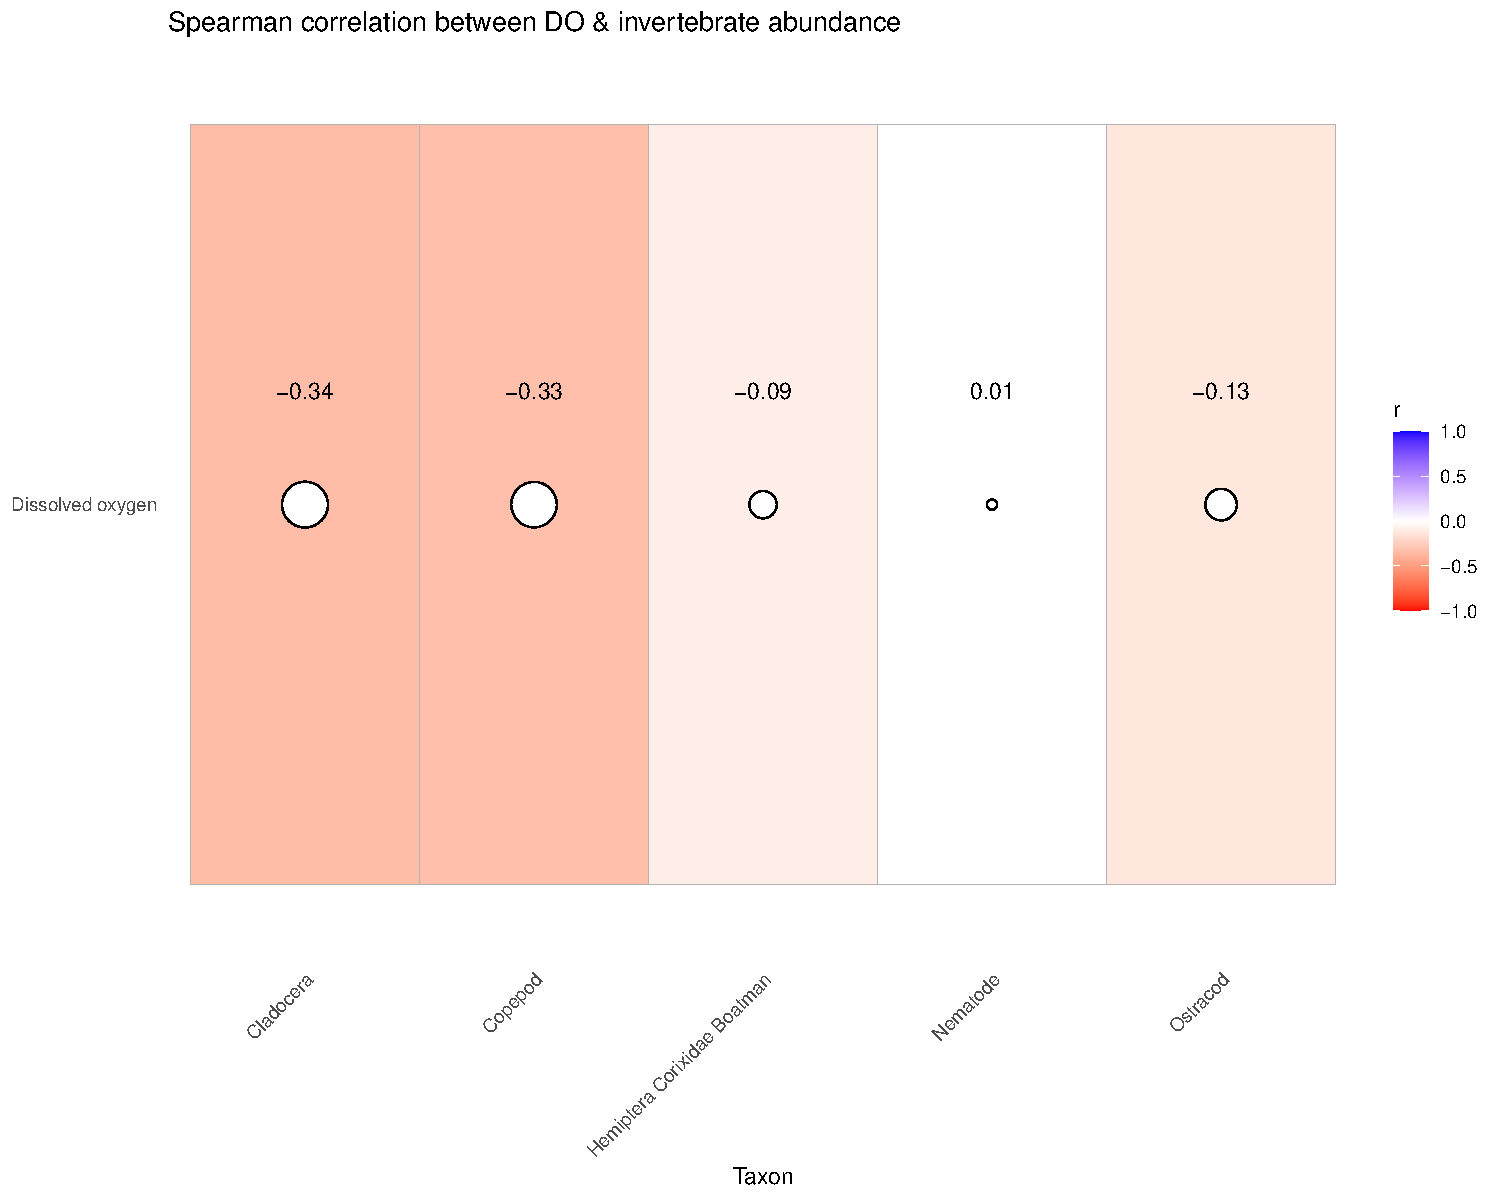
\includegraphics[keepaspectratio]{timeline-check-in_files/figure-pdf/Correlation analysis for Each Focus Taxa and DO levels-1.pdf}}

Most focus taxa showed \textbf{weak negative} correlations with
dissolved oxygen, with Cladocera and Copepod showing the strongest
negative relationships and Nematode showing almost no relationship.

\subsection{Pearson correlation for continuous DO and total community
abundance}\label{pearson-correlation-for-continuous-do-and-total-community-abundance}

\begin{Shaded}
\begin{Highlighting}[]
\CommentTok{\# run a Pearson correlation test between log total abundance + median DO}
\FunctionTok{cor.test}\NormalTok{(}
\NormalTok{  total\_abundance}\SpecialCharTok{$}\NormalTok{log\_total\_abundance, }\CommentTok{\# log total abundance is first variable}
\NormalTok{  total\_abundance}\SpecialCharTok{$}\NormalTok{med\_do, }\CommentTok{\# use median DO as the second variable}
         \AttributeTok{method =} \StringTok{"pearson"}\NormalTok{) }\CommentTok{\# specify pearson method}
\end{Highlighting}
\end{Shaded}

\begin{verbatim}

    Pearson's product-moment correlation

data:  total_abundance$log_total_abundance and total_abundance$med_do
t = -2.2882, df = 32, p-value = 0.02887
alternative hypothesis: true correlation is not equal to 0
95 percent confidence interval:
 -0.63289820 -0.04217141
sample estimates:
       cor 
-0.3749894 
\end{verbatim}

\begin{Shaded}
\begin{Highlighting}[]
\CommentTok{\# r = {-}0.3749894, p = 0.02887}
\CommentTok{\# there is a significant negative correlation between abundance and continous DO}
\end{Highlighting}
\end{Shaded}

There was a \textbf{statistically significant negative linear
relationship} between median dissolved oxygen and log-transformed total
invertebrate abundance, suggesting that abundance decreased as DO
increased.

\subsection{Kruskal-Wallis test comparing abundance across DO
categories}\label{kruskal-wallis-test-comparing-abundance-across-do-categories}

\begin{Shaded}
\begin{Highlighting}[]
\CommentTok{\# run a Kruskal{-}Wallis test comparing log total abundance across DO categories}
\FunctionTok{kruskal.test}\NormalTok{(log\_total\_abundance }\SpecialCharTok{\textasciitilde{}}\NormalTok{ do\_category,}
             \CommentTok{\# use the total\_abundance dataset}
             \AttributeTok{data =}\NormalTok{ total\_abundance)}
\end{Highlighting}
\end{Shaded}

\begin{verbatim}

    Kruskal-Wallis rank sum test

data:  log_total_abundance by do_category
Kruskal-Wallis chi-squared = 2.0001, df = 2, p-value = 0.3679
\end{verbatim}

\begin{Shaded}
\begin{Highlighting}[]
\CommentTok{\# Kruskal{-}Wallis chi{-}squared = 3.2212, df = 2, p{-}value = 0.1998}
\CommentTok{\# there is not a significant difference between abundance and DO categories}
\end{Highlighting}
\end{Shaded}

Total log-transformed invertebrate abundance \textbf{did not differ
significantly} across low, moderate, and high DO categories.

\subsection{Chi-Square}\label{chi-square}

\begin{Shaded}
\begin{Highlighting}[]
\CommentTok{\# create abundance table for chi{-}square test}
\NormalTok{chi\_square\_table }\OtherTok{\textless{}{-}}\NormalTok{ aq\_ins\_clean\_bins }\SpecialCharTok{|\textgreater{}}
  \CommentTok{\# keep only rows with the focus taxa}
  \FunctionTok{filter}\NormalTok{(taxon }\SpecialCharTok{\%in\%}\NormalTok{ focus\_taxa) }\SpecialCharTok{|\textgreater{}}
  \CommentTok{\# group data by DO bin + taxon}
  \FunctionTok{group\_by}\NormalTok{(bins, taxon) }\SpecialCharTok{|\textgreater{}}
  \FunctionTok{summarise}\NormalTok{(}
    \CommentTok{\# sum average abundance per liter + ignore missing values}
    \AttributeTok{total\_abundance =} \FunctionTok{sum}\NormalTok{(ave\_lit, }\AttributeTok{na.rm =} \ConstantTok{TRUE}\NormalTok{),}
    \CommentTok{\# ungroup}
    \AttributeTok{.groups =} \StringTok{"drop"}\NormalTok{) }\SpecialCharTok{|\textgreater{}}
  \CommentTok{\# convert the table from long format to wide format}
  \FunctionTok{pivot\_wider}\NormalTok{(}
    \CommentTok{\# create one column for each taxon}
    \AttributeTok{names\_from =}\NormalTok{ taxon,}
    \CommentTok{\# fill taxon columns with total abundance values}
    \AttributeTok{values\_from =}\NormalTok{ total\_abundance,}
    \CommentTok{\# fill missing values with 0}
    \AttributeTok{values\_fill =} \DecValTok{0}\NormalTok{) }\SpecialCharTok{|\textgreater{}}
  \CommentTok{\# convert the bins column into row names}
  \FunctionTok{column\_to\_rownames}\NormalTok{(}\StringTok{"bins"}\NormalTok{) }\SpecialCharTok{|\textgreater{}}
  \CommentTok{\# convert the table into a matrix}
  \FunctionTok{as.matrix}\NormalTok{()}

\CommentTok{\# show table}
\NormalTok{chi\_square\_table}
\end{Highlighting}
\end{Shaded}

\begin{verbatim}
         Cladocera   Copepod Hemiptera Corixidae Boatman  Nematode    Ostracod
low       980.2667  115.8667                   0.2666667 0.1333333 1202.933333
moderate  510.6667 1170.4000                  83.8666667 0.2666667 1057.866667
high      264.2667 1453.4667                   8.8000000 0.0000000    7.866667
\end{verbatim}

\begin{Shaded}
\begin{Highlighting}[]
\CommentTok{\# chi{-}square test for differences in taxon composition across DO bins}
\NormalTok{chi\_square\_test }\OtherTok{\textless{}{-}} \FunctionTok{chisq.test}\NormalTok{(chi\_square\_table)}

\CommentTok{\# show chi{-}square result}
\NormalTok{chi\_square\_test}
\end{Highlighting}
\end{Shaded}

\begin{verbatim}

    Pearson's Chi-squared test

data:  chi_square_table
X-squared = 2859.2, df = 8, p-value < 2.2e-16
\end{verbatim}

Taxon composition \textbf{differed significantly across DO bins},
suggesting that the invertebrate community structure changes depending
on dissolved oxygen category.

\section{Visualizations directly relevant to answering
questions}\label{visualizations-directly-relevant-to-answering-questions}

\subsection{Directly Relevant Figure 1: DO levels vs invert. abundance
for each focus
taxa}\label{directly-relevant-figure-1-do-levels-vs-invert.-abundance-for-each-focus-taxa}

\begin{Shaded}
\begin{Highlighting}[]
\CommentTok{\# creates object DO\_taxa\_medians from DO\_taxa}
\NormalTok{DO\_taxa\_medians }\OtherTok{\textless{}{-}}\NormalTok{ DO\_taxa }\SpecialCharTok{|\textgreater{}}
  \CommentTok{\# groups data by taxon so each species gets one median point}
  \FunctionTok{group\_by}\NormalTok{(taxon) }\SpecialCharTok{|\textgreater{}}
  \CommentTok{\# calculates median DO and median log abundance for each taxon}
  \FunctionTok{summarise}\NormalTok{(}
    \CommentTok{\# calculates the median DO value for each taxon}
    \AttributeTok{med\_do\_point =} \FunctionTok{median}\NormalTok{(med\_do, }\AttributeTok{na.rm =} \ConstantTok{TRUE}\NormalTok{),}
    \CommentTok{\# calculates the median log{-}transformed average abundance for each taxon}
    \AttributeTok{med\_log\_ave\_lit =} \FunctionTok{median}\NormalTok{(log\_ave\_lit, }\AttributeTok{na.rm =} \ConstantTok{TRUE}\NormalTok{),}
    \CommentTok{\# ungroup}
    \AttributeTok{.groups =} \StringTok{"drop"}\NormalTok{)}
\end{Highlighting}
\end{Shaded}

\begin{Shaded}
\begin{Highlighting}[]
\NormalTok{DO\_taxa\_plot }\OtherTok{\textless{}{-}} \FunctionTok{ggplot}\NormalTok{(}\AttributeTok{data =}\NormalTok{ DO\_taxa, }\CommentTok{\# assigns plot to object do\_taxa\_plot }
                        \CommentTok{\# uses DO\_taxa data frame}
                        \AttributeTok{mapping =} \FunctionTok{aes}\NormalTok{(}\AttributeTok{x =}\NormalTok{ med\_do, }\CommentTok{\# x{-}axis: med\_do}
                                      \AttributeTok{y =}\NormalTok{ log\_ave\_lit, }\CommentTok{\# y{-}axis: log\_ave\_lit}
                                      \AttributeTok{color =}\NormalTok{ taxon)) }\SpecialCharTok{+} \CommentTok{\# color by taxon}
  \CommentTok{\# first layer: points show individual abundance measurements }
  \FunctionTok{geom\_point}\NormalTok{(}\AttributeTok{shape =} \DecValTok{16}\NormalTok{, }\CommentTok{\# shape is circle}
             \AttributeTok{size =} \DecValTok{2}\NormalTok{, }\CommentTok{\# size is 2}
             \AttributeTok{alpha =} \FloatTok{0.7}\NormalTok{) }\SpecialCharTok{+} \CommentTok{\# opacity is 0.7}
  \CommentTok{\# second layer: larger point shows the median location for each taxon}
  \FunctionTok{geom\_point}\NormalTok{(}\AttributeTok{data =}\NormalTok{ DO\_taxa\_medians,}
             \AttributeTok{mapping =} \FunctionTok{aes}\NormalTok{(}\AttributeTok{x =}\NormalTok{ med\_do\_point, }\CommentTok{\# x value is median DO}
                           \CommentTok{\# y value is median log{-}transformed abundance}
                           \AttributeTok{y =}\NormalTok{ med\_log\_ave\_lit),}
             \AttributeTok{shape =} \DecValTok{18}\NormalTok{, }\CommentTok{\# makes shape of points diamond}
             \AttributeTok{size =} \DecValTok{5}\NormalTok{) }\SpecialCharTok{+} \CommentTok{\# size of points is 5}
  \CommentTok{\# separate panels for each taxon with free x{-} and y{-}axis scales}
  \FunctionTok{facet\_wrap}\NormalTok{(}\SpecialCharTok{\textasciitilde{}}\NormalTok{ taxon, }\AttributeTok{scales =} \StringTok{"free"}\NormalTok{) }\SpecialCharTok{+}
  \CommentTok{\# use non{-}default colors for points}
  \FunctionTok{scale\_color\_viridis\_d}\NormalTok{() }\SpecialCharTok{+}
  \FunctionTok{labs}\NormalTok{(}\AttributeTok{x =} \StringTok{"Median DO (mg/L)"}\NormalTok{, }\CommentTok{\# relabel x{-}axis}
       \AttributeTok{y =} \StringTok{"log + 1 transformed average abundance/L"}\NormalTok{, }\CommentTok{\# relabel y{-}axis}
       \CommentTok{\# creates descriptive title}
       \AttributeTok{title =} \StringTok{"Invertebrate abundance as a function of DO"}\NormalTok{) }\SpecialCharTok{+}
  \CommentTok{\# uses non{-}default theme}
  \FunctionTok{theme\_minimal}\NormalTok{() }\SpecialCharTok{+}
  \CommentTok{\# remove redundant legend}
  \FunctionTok{theme}\NormalTok{(}\AttributeTok{legend.position =} \StringTok{"none"}\NormalTok{)}
\CommentTok{\# shows plot}
\NormalTok{DO\_taxa\_plot}
\end{Highlighting}
\end{Shaded}

\pandocbounded{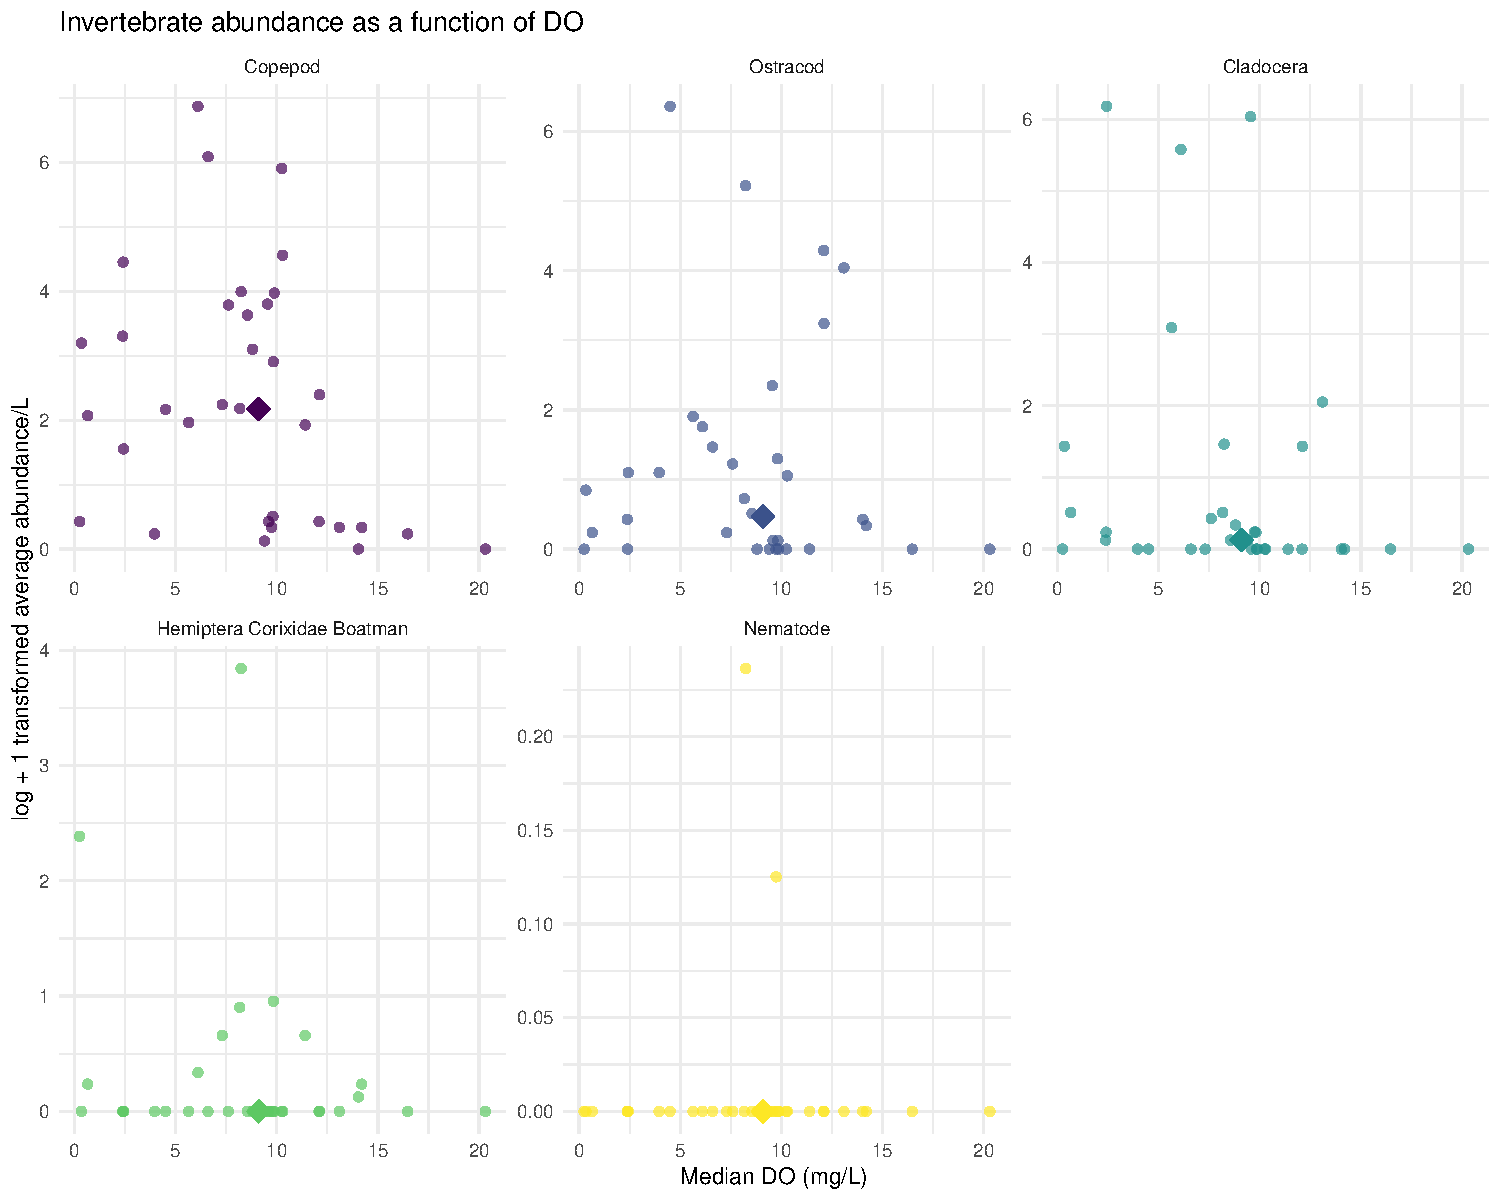
\includegraphics[keepaspectratio]{timeline-check-in_files/figure-pdf/figure 1 - DO_taxa_plot-1.pdf}}

Description of visual components

This figure shows the relationship between Median DO (mg/L) and log + 1
transformed average invertebrate abundance/L for our five focus taxa.
Each panel represents a different taxon. Each small point represents one
observation of that taxon, with median dissolved oxygen shown on the
x-axis in mg/L and log + 1 transformed average abundance per liter shown
on the y-axis. The different colors distinguish the taxa, and the larger
diamond in each panel represents the overall average/summary point for
that taxon across observations.

Main message / takeaway

Overall, there does not appear to be a strong or consistent relationship
between median dissolved oxygen and invertebrate abundance across all
taxa. Some taxa, especially Copepods, Ostracods, and Cladocerans, show
higher abundances at low to moderate dissolved oxygen levels, but the
pattern is variable and differs by taxon.

Connection to the main question

This figure helps evaluate whether dissolved oxygen is related to
invertebrate abundance in the study system. The variation among taxa
suggests that dissolved oxygen may influence some invertebrate groups
differently, but DO alone does not clearly explain abundance patterns
across the full invertebrate community.

\subsection{Directly Relevant Figure 2: DO levels vs total invert.
abundance}\label{directly-relevant-figure-2-do-levels-vs-total-invert.-abundance}

\begin{Shaded}
\begin{Highlighting}[]
\CommentTok{\# fit linear model for relationship between log abundance and median DO}
\NormalTok{total\_abundance\_lm }\OtherTok{\textless{}{-}} \FunctionTok{lm}\NormalTok{(log\_total\_abundance }\SpecialCharTok{\textasciitilde{}}\NormalTok{ med\_do, }
                         \CommentTok{\# use total\_abundance as df}
                         \AttributeTok{data =}\NormalTok{ total\_abundance)}

\CommentTok{\# create new data frame total\_abundance\_predictions for predicted values}
\NormalTok{total\_abundance\_predictions }\OtherTok{\textless{}{-}} \FunctionTok{data.frame}\NormalTok{( }
  \CommentTok{\# create a sequence of DO values from the minimum to maximum observed DO}
  \AttributeTok{med\_do =} \FunctionTok{seq}\NormalTok{(}\FunctionTok{min}\NormalTok{(total\_abundance}\SpecialCharTok{$}\NormalTok{med\_do, }\AttributeTok{na.rm =} \ConstantTok{TRUE}\NormalTok{), }\CommentTok{\# max value is max DO}
               \FunctionTok{max}\NormalTok{(total\_abundance}\SpecialCharTok{$}\NormalTok{med\_do, }\AttributeTok{na.rm =} \ConstantTok{TRUE}\NormalTok{), }\CommentTok{\# min value is min DO}
               \CommentTok{\# creates 100 evenly spaced values for smooth predictions}
               \AttributeTok{length.out =} \DecValTok{100}\NormalTok{))}

\CommentTok{\# generate predicted values and confidence intervals}
\NormalTok{total\_abundance\_predictions }\OtherTok{\textless{}{-}}\NormalTok{ total\_abundance\_predictions }\SpecialCharTok{|\textgreater{}}
  \FunctionTok{bind\_cols}\NormalTok{( }\CommentTok{\# attach model predictions + confidence interval values to df}
    \CommentTok{\# predict log total abundance using the fitted linear model}
    \FunctionTok{predict}\NormalTok{(total\_abundance\_lm, }
            \CommentTok{\# use the total\_abundance\_predictions df as data for prediction}
            \AttributeTok{newdata =}\NormalTok{ total\_abundance\_predictions,}
            \CommentTok{\# create confidence intervals around the fitted values}
            \AttributeTok{interval =} \StringTok{"confidence"}\NormalTok{) }\SpecialCharTok{|\textgreater{}}
      \CommentTok{\# convert prediction output into a data frame}
      \FunctionTok{as.data.frame}\NormalTok{())}

\CommentTok{\# creat plot from total\_abundance df}
\FunctionTok{ggplot}\NormalTok{(total\_abundance,}
       \FunctionTok{aes}\NormalTok{(}\AttributeTok{x =}\NormalTok{ med\_do, }\CommentTok{\# x{-}axis is total\_abundance}
           \AttributeTok{y =}\NormalTok{ log\_total\_abundance)) }\SpecialCharTok{+} \CommentTok{\# y{-}axis is log\_total\_abundance}
  \CommentTok{\# layer 1: create points  }
  \FunctionTok{geom\_point}\NormalTok{(}\AttributeTok{color =} \StringTok{"magenta3"}\NormalTok{, }\CommentTok{\# color points}
             \AttributeTok{size =} \DecValTok{3}\NormalTok{, }\CommentTok{\# size of points is 3}
             \AttributeTok{alpha =} \FloatTok{0.7}\NormalTok{) }\SpecialCharTok{+} \CommentTok{\# opacity of points is 0.7}
  \CommentTok{\# layer 2: creates ribbon confidence interval around model predictions}
  \FunctionTok{geom\_ribbon}\NormalTok{(}\AttributeTok{data =}\NormalTok{ total\_abundance\_predictions, }
              \FunctionTok{aes}\NormalTok{(}\AttributeTok{x =}\NormalTok{ med\_do, }\CommentTok{\# x is median DO}
                  \AttributeTok{ymin =}\NormalTok{ lwr, }\CommentTok{\# min on y is lower confidence interval}
                  \AttributeTok{ymax =}\NormalTok{ upr), }\CommentTok{\# max on y is lower confidence interval}
              \AttributeTok{inherit.aes =} \ConstantTok{FALSE}\NormalTok{, }\CommentTok{\# does not inherit ggplot aesthetics}
              \AttributeTok{fill =} \StringTok{"cyan2"}\NormalTok{, }\CommentTok{\# colors ribbon}
              \AttributeTok{alpha =} \FloatTok{0.35}\NormalTok{) }\SpecialCharTok{+} \CommentTok{\# opacity of points is 0.35}
  \CommentTok{\# layer 3: creates predicted line from linear model}
  \FunctionTok{geom\_line}\NormalTok{(}\AttributeTok{data =}\NormalTok{ total\_abundance\_predictions, }
            \FunctionTok{aes}\NormalTok{(}\AttributeTok{x =}\NormalTok{ med\_do, }\CommentTok{\# x is median DO}
                \AttributeTok{y =}\NormalTok{ fit), }\CommentTok{\# y is fitted model values}
            \AttributeTok{inherit.aes =} \ConstantTok{FALSE}\NormalTok{,  }\CommentTok{\# does not inherit ggplot aesthetics}
            \AttributeTok{color =} \StringTok{"purple4"}\NormalTok{, }\CommentTok{\# colors prediction line}
            \AttributeTok{linewidth =} \DecValTok{1}\NormalTok{) }\SpecialCharTok{+} \CommentTok{\# sets line width}
  \FunctionTok{labs}\NormalTok{(}
    \AttributeTok{x =} \StringTok{"Dissolved oxygen (mg/L)"}\NormalTok{, }\CommentTok{\# labels x{-}axis}
    \AttributeTok{y =} \StringTok{"Log total invertebrate abundance"}\NormalTok{, }\CommentTok{\# labels y{-}axis}
    \CommentTok{\# creates descriptive title}
    \AttributeTok{title =} \StringTok{"Relationship between DO + total invertebrate abundance"}\NormalTok{) }\SpecialCharTok{+}
  \CommentTok{\# uses non{-}default theme}
  \FunctionTok{theme\_classic}\NormalTok{()}
\end{Highlighting}
\end{Shaded}

\pandocbounded{\includegraphics[keepaspectratio]{timeline-check-in_files/figure-pdf/figure 2 - DO levels vs total invert. abundance-1.pdf}}

\begin{Shaded}
\begin{Highlighting}[]
\CommentTok{\# show the linear model results in a tidy table format}
\NormalTok{broom}\SpecialCharTok{::}\FunctionTok{tidy}\NormalTok{(total\_abundance\_lm)}
\end{Highlighting}
\end{Shaded}

\begin{verbatim}
# A tibble: 2 x 5
  term        estimate std.error statistic     p.value
  <chr>          <dbl>     <dbl>     <dbl>       <dbl>
1 (Intercept)   2.01      0.302       6.65 0.000000170
2 med_do       -0.0723    0.0316     -2.29 0.0289     
\end{verbatim}

Description of visual components

This figure shows the relationship between DO and total invertebrate
abundance summed across our five focus taxa. Each pink point represents
one sampling observation grouped by date, site, and median dissolved
oxygen, where abundance was summed across the focus taxa and then
log-transformed using log10(total\_abundance + 1). The x-axis shows
median dissolved oxygen in mg/L, and the y-axis shows log-transformed
total invertebrate abundance. The purple line represents the predicted
relationship from a linear model, and the light blue shaded area
represents the confidence interval around the model prediction.

Main message / takeaway

The figure shows a negative relationship between DO and total
invertebrate abundance, where total invertebrate abundance tends to
decrease as dissolved oxygen increases. However, there is still
noticeable variation around the trend line, so dissolved oxygen explains
some, but not all, of the variation in total abundance.

Connection to the main question

This figure directly addresses whether dissolved oxygen is related to
invertebrate abundance by combining the focus taxa into one
community-level abundance measure. It helps contextualize the main
question by showing that lower dissolved oxygen conditions are
associated with higher invertebrate abundance in this dataset.

\subsection{Directly Relevant Figure 3: Abundance vs DO with binned
levels}\label{directly-relevant-figure-3-abundance-vs-do-with-binned-levels}

\begin{Shaded}
\begin{Highlighting}[]
\FunctionTok{ggplot}\NormalTok{(total\_abundance, }\CommentTok{\# uses total\_abundance df}
       \FunctionTok{aes}\NormalTok{(}\AttributeTok{x =}\NormalTok{ do\_category, }\CommentTok{\# x{-}axis is do\_category}
           \AttributeTok{y =}\NormalTok{ log\_total\_abundance, }\CommentTok{\# y{-}axis is log\_total\_abundance}
           \AttributeTok{fill =}\NormalTok{ do\_category)) }\SpecialCharTok{+} \CommentTok{\# fill color by do\_category}
  \CommentTok{\# layer 1: add boxplots to summarize abundance distribution w/in each DO level }
  \FunctionTok{geom\_boxplot}\NormalTok{(}\AttributeTok{alpha =} \FloatTok{0.7}\NormalTok{, }\CommentTok{\# transparency is 0.7}
               \AttributeTok{outlier.color =} \StringTok{"red"}\NormalTok{, }\CommentTok{\# color outlier points red}
               \AttributeTok{outlier.size =} \DecValTok{2}\NormalTok{) }\SpecialCharTok{+} \CommentTok{\# outlier size is 2}
  \CommentTok{\# layer 2: adds jittered points of raw data}
  \FunctionTok{geom\_jitter}\NormalTok{(}\AttributeTok{width =} \FloatTok{0.15}\NormalTok{, }\CommentTok{\# sets point width}
              \AttributeTok{alpha =} \FloatTok{0.5}\NormalTok{, }\CommentTok{\# sets point opacity}
              \AttributeTok{size =} \DecValTok{2}\NormalTok{, }\CommentTok{\# sets point size}
              \AttributeTok{color =} \StringTok{"black"}\NormalTok{) }\SpecialCharTok{+} \CommentTok{\# sets point color}
  \FunctionTok{labs}\NormalTok{(}
    \AttributeTok{x =} \StringTok{"Dissolved oxygen level"}\NormalTok{, }\CommentTok{\# labels x{-}axis}
    \AttributeTok{y =} \StringTok{"Log total invertebrate abundance"}\NormalTok{, }\CommentTok{\# labels y{-}axis}
    \CommentTok{\# creates descriptive title}
    \AttributeTok{title =} \StringTok{"Invertebrate abundance across dissolved oxygen levels"}\NormalTok{) }\SpecialCharTok{+}
  \CommentTok{\# manually assign fill colors to each DO category}
  \FunctionTok{scale\_fill\_manual}\NormalTok{(}\AttributeTok{values =} \FunctionTok{c}\NormalTok{(}
    \StringTok{"Low DO"} \OtherTok{=} \StringTok{"red3"}\NormalTok{, }\CommentTok{\# set Low DO color}
    \StringTok{"Medium DO"} \OtherTok{=} \StringTok{"grey60"}\NormalTok{, }\CommentTok{\# set Medium DO color}
    \StringTok{"High DO"} \OtherTok{=} \StringTok{"blue3"}\NormalTok{)) }\SpecialCharTok{+} \CommentTok{\# set High DO color}
  \CommentTok{\# uses non{-}default theme}
  \FunctionTok{theme\_classic}\NormalTok{() }\SpecialCharTok{+}
  \CommentTok{\# removes redundant legend}
  \FunctionTok{theme}\NormalTok{(}\AttributeTok{legend.position =} \StringTok{"none"}\NormalTok{)}
\end{Highlighting}
\end{Shaded}

\pandocbounded{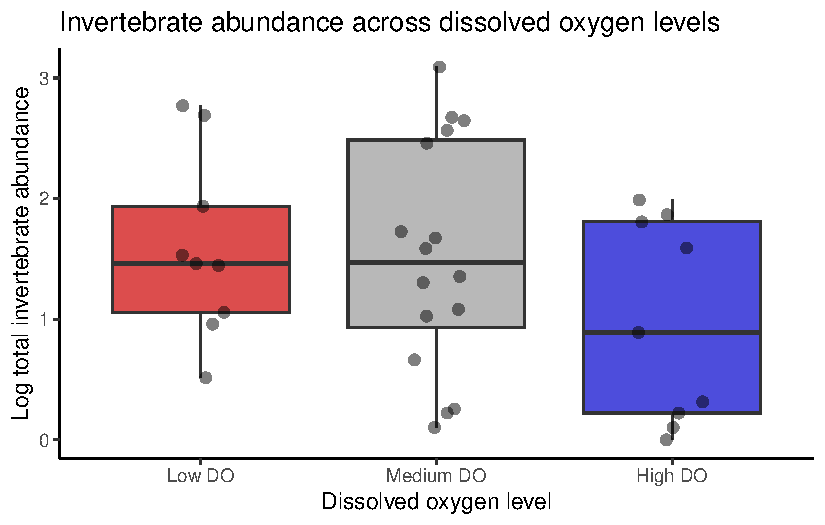
\includegraphics[keepaspectratio]{timeline-check-in_files/figure-pdf/figure 3 - Abundance vs DO with binned levels-1.pdf}}

Description of visual components

This figure compares log-transformed total invertebrate abundance across
three DO categories: Low DO, Medium DO, and High DO. Each black jittered
point represents one sampling observation grouped by date, site, and
median dissolved oxygen, where abundance was summed across the five
focus taxa and transformed using log10(total\_abundance + 1). The
colored boxes show the middle 50\% of abundance values for each DO
category, the thick horizontal line inside each box represents the
median, and the whiskers show the spread of values outside the
interquartile range.

Main message / takeaway

Total invertebrate abundance appears lower in the High DO category
compared with the Low DO and Medium DO categories. However, there is
substantial overlap and variability among the DO categories, especially
in the Medium DO group, so the difference is not extremely clear-cut
from the visualization alone.

Connection to the main question

This figure helps address whether invertebrate abundance differs across
dissolved oxygen levels by grouping continuous DO values into low,
medium, and high categories. It shows that total invertebrate abundance
may be higher under low-to-medium DO conditions and lower under high DO
conditions in this dataset.

\section{Other exploratory
visualizations}\label{other-exploratory-visualizations}

\subsection{Exploratory Figure 1: Variance of DO across
sights}\label{exploratory-figure-1-variance-of-do-across-sights}

\begin{Shaded}
\begin{Highlighting}[]
\CommentTok{\# create object aq\_ins\_clean\_fig2 from aq\_ins\_clean}
\NormalTok{aq\_ins\_clean\_fig2 }\OtherTok{\textless{}{-}}\NormalTok{  aq\_ins\_clean }\SpecialCharTok{|\textgreater{}}
  \CommentTok{\# convert taxon to title case}
  \FunctionTok{mutate}\NormalTok{(}\AttributeTok{taxon =} \FunctionTok{str\_replace\_all}\NormalTok{(taxon, }\StringTok{"\_"}\NormalTok{, }\StringTok{" "}\NormalTok{), }\AttributeTok{taxon =} \FunctionTok{str\_to\_title}\NormalTok{(taxon)) }\SpecialCharTok{|\textgreater{}} 
  \CommentTok{\# filter to only include focus taxa}
  \FunctionTok{filter}\NormalTok{(taxon }\SpecialCharTok{\%in\%}\NormalTok{ focus\_taxa)}

\CommentTok{\# base layer create plot from aq\_ins\_clean\_fig2 df}
\NormalTok{DO }\OtherTok{\textless{}{-}} \FunctionTok{ggplot}\NormalTok{(}\AttributeTok{data =}\NormalTok{ aq\_ins\_clean\_fig2,}
       \AttributeTok{mapping =} \FunctionTok{aes}\NormalTok{(}\AttributeTok{x =}\NormalTok{ site\_full, }\CommentTok{\# x{-}axis: site}
                     \AttributeTok{y =}\NormalTok{ med\_do)) }\SpecialCharTok{+} \CommentTok{\# y{-}axis: mean salinity}
  \CommentTok{\# first layer: boxplot}
  \FunctionTok{geom\_boxplot}\NormalTok{(}\AttributeTok{width =} \FloatTok{0.35}\NormalTok{, }\AttributeTok{outlier.shape =} \ConstantTok{NA}\NormalTok{) }\SpecialCharTok{+}
  \CommentTok{\# second layer: jittered points for salinity measurements}
  \FunctionTok{geom\_jitter}\NormalTok{(}\AttributeTok{height =} \DecValTok{0}\NormalTok{, }\CommentTok{\# sets height of jitter}
              \AttributeTok{width =} \FloatTok{0.12}\NormalTok{, }\CommentTok{\# sets width of jitter}
              \AttributeTok{shape =} \DecValTok{21}\NormalTok{, }\CommentTok{\# sets shape of jittered points}
              \AttributeTok{alpha =} \FloatTok{0.6}\NormalTok{) }\SpecialCharTok{+} \CommentTok{\# sets opacity of jittered points}
  \CommentTok{\# wrapping x{-}axis text for readability}
  \FunctionTok{scale\_x\_discrete}\NormalTok{(}\AttributeTok{labels =} \FunctionTok{label\_wrap}\NormalTok{(}\AttributeTok{width =} \DecValTok{15}\NormalTok{)) }\SpecialCharTok{+}
  \CommentTok{\# second layer: points to represent medians}
  \FunctionTok{stat\_summary}\NormalTok{(}\AttributeTok{fun =}\NormalTok{ median, }\CommentTok{\# function is median value}
               \AttributeTok{color =} \StringTok{"red"}\NormalTok{, }\CommentTok{\# colors median points}
               \AttributeTok{size =} \DecValTok{1}\NormalTok{) }\SpecialCharTok{+} \CommentTok{\# sets size of median points}
  \FunctionTok{labs}\NormalTok{(}\AttributeTok{x =} \StringTok{"Site"}\NormalTok{, }\CommentTok{\# labels x{-}axis}
       \AttributeTok{y =} \StringTok{"Median DO (mg/L)"}\NormalTok{, }\CommentTok{\# labels y{-}axis}
       \AttributeTok{title =} \StringTok{"Site DO levels"}\NormalTok{) }\SpecialCharTok{+} \CommentTok{\# creates descriptive title}
  \CommentTok{\# uses non{-}default theme}
  \FunctionTok{theme\_bw}\NormalTok{()}

\CommentTok{\# shows plot}
\NormalTok{DO}
\end{Highlighting}
\end{Shaded}

\pandocbounded{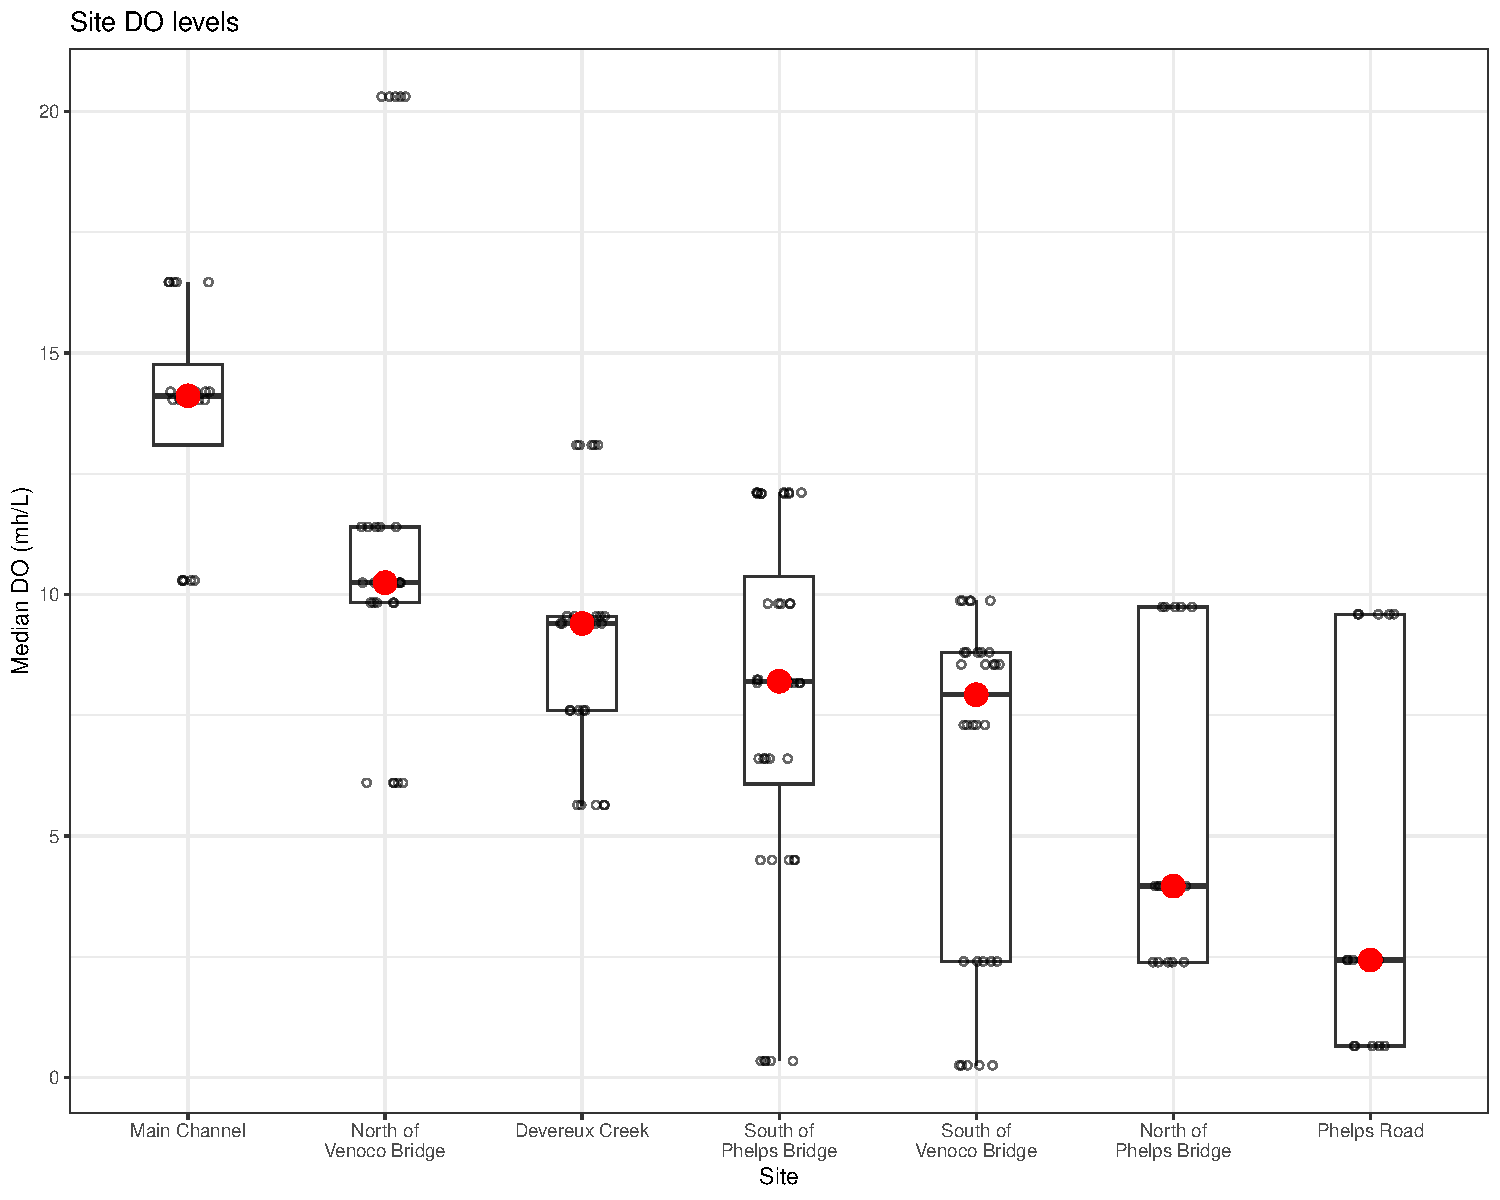
\includegraphics[keepaspectratio]{timeline-check-in_files/figure-pdf/exp. figure 1 - Variance of DO across sights-1.pdf}}

Description of visual components

This figure shows how median DO varies across sampling sites. Each
jittered open point represents one observation of median DO at a site,
based on the focus invertebrate sampling data. The boxplots summarize
the distribution of DO values at each site, where the box shows the IQR
and the horizontal line inside the box shows the median. The large red
point marks the median DO value for each site.

Main message / takeaway

There are clear differences in dissolved oxygen among sites. Main
Channel has the highest DO values overall, while North of Phelps Bridge
and Phelps Road tend to have the lowest DO values, with the other sites
showing intermediate conditions.

Connection to the main question

This figure helps contextualize the main question by showing that
dissolved oxygen is not uniform across the study area, and varies
substantially by site. These differences in DO between sites may help
explain patterns in invertebrate abundance, since organisms at different
sites are experiencing different oxygen conditions.

\subsection{Exploratory Figure 2: Composition plot across DO
bins}\label{exploratory-figure-2-composition-plot-across-do-bins}

\begin{Shaded}
\begin{Highlighting}[]
\CommentTok{\# creates obejct composition\_plot using DO\_taxa df}
\NormalTok{composition\_plot }\OtherTok{\textless{}{-}}\NormalTok{ DO\_taxa }\SpecialCharTok{|\textgreater{}} 
  \FunctionTok{mutate}\NormalTok{(}
    \CommentTok{\# classify each observation into low, medium, or high dissolved oxygen}
    \AttributeTok{do\_category =} \FunctionTok{case\_when}\NormalTok{(}
      \CommentTok{\# assign Low DO to values at or below the 25th percentile of median DO}
\NormalTok{      med\_do }\SpecialCharTok{\textless{}=} \FunctionTok{quantile}\NormalTok{(med\_do, }\FloatTok{0.25}\NormalTok{, }\AttributeTok{na.rm =} \ConstantTok{TRUE}\NormalTok{) }\SpecialCharTok{\textasciitilde{}} \StringTok{"Low DO"}\NormalTok{,}
      \CommentTok{\# assign Medium DO to values between the 25th percentile {-} 75th percentile}
\NormalTok{      med\_do }\SpecialCharTok{\textless{}=} \FunctionTok{quantile}\NormalTok{(med\_do, }\FloatTok{0.75}\NormalTok{, }\AttributeTok{na.rm =} \ConstantTok{TRUE}\NormalTok{) }\SpecialCharTok{\textasciitilde{}} \StringTok{"Medium DO"}\NormalTok{,}
      \CommentTok{\# assign High DO to all remaining values above the 75th percentile}
      \ConstantTok{TRUE} \SpecialCharTok{\textasciitilde{}} \StringTok{"High DO"}\NormalTok{),}
    \CommentTok{\# convert do\_category into a factor to control plotting order}
    \AttributeTok{do\_category =} \FunctionTok{factor}\NormalTok{(do\_category,}
                         \CommentTok{\# set order of DO categories on the x{-}axis}
                         \AttributeTok{levels =} \FunctionTok{c}\NormalTok{(}\StringTok{"Low DO"}\NormalTok{, }\StringTok{"Medium DO"}\NormalTok{, }\StringTok{"High DO"}\NormalTok{))) }\SpecialCharTok{|\textgreater{}}
  \CommentTok{\# groups by do\_category and taxon}
  \FunctionTok{group\_by}\NormalTok{(do\_category, taxon) }\SpecialCharTok{|\textgreater{}}
  \CommentTok{\# calculate total abundance for each taxon within each DO category}
  \FunctionTok{summarize}\NormalTok{(}
    \CommentTok{\# sum average abundance per liter + ignore missing values}
    \AttributeTok{total\_abundance =} \FunctionTok{sum}\NormalTok{(ave\_lit, }\AttributeTok{na.rm =} \ConstantTok{TRUE}\NormalTok{),}
    \CommentTok{\# ungroup}
    \AttributeTok{.groups =} \StringTok{"drop"}\NormalTok{) }\SpecialCharTok{|\textgreater{}}

\CommentTok{\# create plot from composition\_plot df}
\FunctionTok{ggplot}\NormalTok{(}\FunctionTok{aes}\NormalTok{(}\AttributeTok{x =}\NormalTok{ do\_category, }\CommentTok{\# x{-}axis is do\_category}
           \AttributeTok{y =}\NormalTok{ total\_abundance, }\CommentTok{\# y{-}axis is total\_abundance}
           \AttributeTok{fill =}\NormalTok{ taxon)) }\SpecialCharTok{+} \CommentTok{\# fill color by taxon}
  \CommentTok{\# create stacked bars scaled to proportions within each DO category}
  \FunctionTok{geom\_col}\NormalTok{(}\AttributeTok{position =} \StringTok{"fill"}\NormalTok{) }\SpecialCharTok{+} 
  \CommentTok{\# format the y{-}axis as percentages}
  \FunctionTok{scale\_y\_continuous}\NormalTok{(}\AttributeTok{labels =}\NormalTok{ scales}\SpecialCharTok{::}\FunctionTok{percent\_format}\NormalTok{()) }\SpecialCharTok{+}
  \FunctionTok{labs}\NormalTok{(}
    \AttributeTok{x =} \StringTok{"Dissolved oxygen category"}\NormalTok{, }\CommentTok{\# relabels x{-}axis}
    \AttributeTok{y =} \StringTok{"Relative community composition"}\NormalTok{, }\CommentTok{\# relabels y{-}axis}
    \AttributeTok{fill =} \StringTok{"Taxon"}\NormalTok{, }\CommentTok{\# labels legend}
    \AttributeTok{title =} \StringTok{"Invertebrate community composition shifts across dissolved oxygen levels"}
\NormalTok{  ) }\SpecialCharTok{+}
  \FunctionTok{theme\_classic}\NormalTok{()}

\NormalTok{composition\_plot}
\end{Highlighting}
\end{Shaded}

\pandocbounded{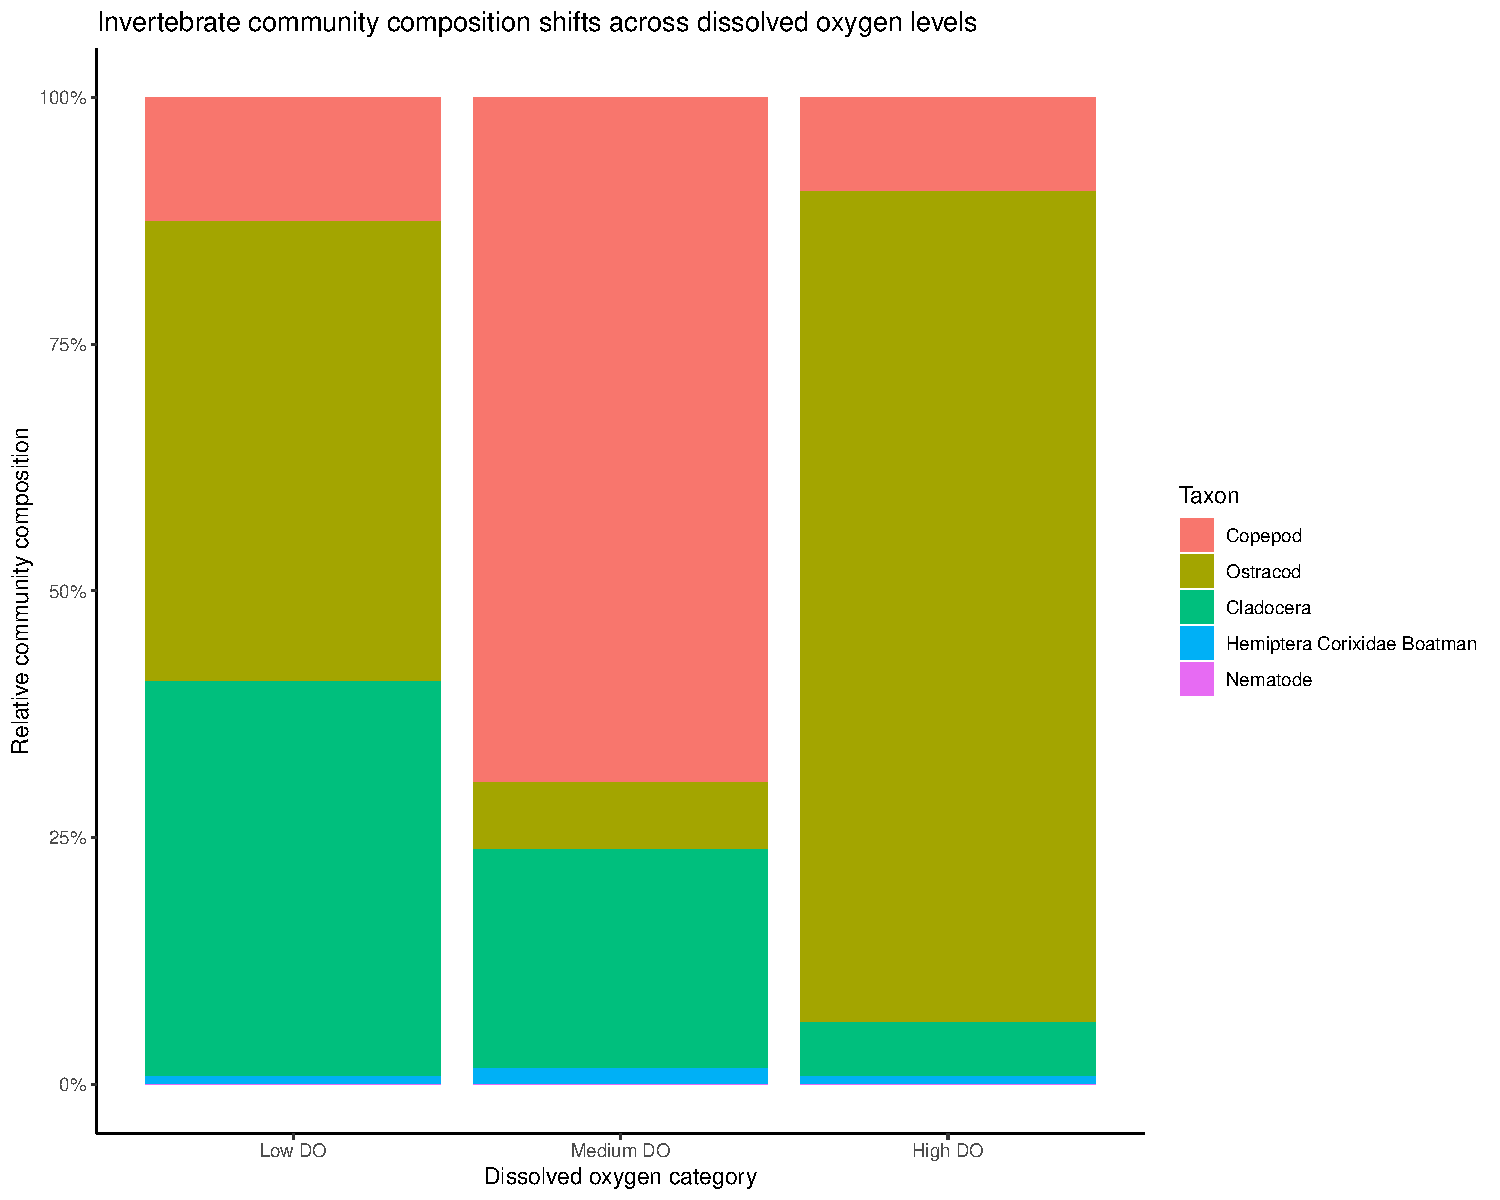
\includegraphics[keepaspectratio]{timeline-check-in_files/figure-pdf/exp. figure 2 - Composition plot across DO bins-1.pdf}}

Description of visual components

This figure shows how relative invertebrate community composition
changes across three dissolved oxygen categories: Low DO, Medium DO, and
High DO. Each stacked bar represents the total abundance of the focus
taxa within one DO category, scaled to 100\% so that the bar shows
relative composition rather than raw abundance. Each colored segment
within a bar represents the proportion contributed by one focus taxon
and the y-axis shows the percent of the community made up by each group.

Main message / takeaway

The figure suggests that invertebrate community composition shifts
across dissolved oxygen levels. Low DO sites have a more mixed community
with large contributions from Cladocera and Ostracods, Medium DO sites
are dominated by Copepods, and High DO sites are dominated primarily by
Ostracods, while Hemiptera Corixidae Boatman and Nematodes remain minor
components across all DO levels.

Connection to the main question

This figure helps address the main question by showing that dissolved
oxygen may influence not only total invertebrate abundance, but also
which taxa make up the community. It provides important context by
suggesting that changes in oxygen conditions are associated with shifts
in community structure, meaning different invertebrate groups may
respond to different DO levels.

\subsection{Exploratory Figure 3: Time-series plot of total abundance
(all
species)}\label{exploratory-figure-3-time-series-plot-of-total-abundance-all-species}

\begin{Shaded}
\begin{Highlighting}[]
\CommentTok{\# create total abundance over time}
\NormalTok{total\_abundance\_time }\OtherTok{\textless{}{-}}\NormalTok{ DO\_taxa }\SpecialCharTok{|\textgreater{}}
  \CommentTok{\# keeps only the taxa of interest}
  \FunctionTok{filter}\NormalTok{(taxon }\SpecialCharTok{\%in\%}\NormalTok{ focus\_taxa) }\SpecialCharTok{|\textgreater{}}
  \CommentTok{\# makes sure date is treated as a date object}
  \FunctionTok{mutate}\NormalTok{(}\AttributeTok{date =} \FunctionTok{as.Date}\NormalTok{(date)) }\SpecialCharTok{|\textgreater{}}
  \CommentTok{\# creates a month column so close sampling dates are summarized together}
  \FunctionTok{mutate}\NormalTok{(}\AttributeTok{month =}\NormalTok{ lubridate}\SpecialCharTok{::}\FunctionTok{floor\_date}\NormalTok{(date, }\AttributeTok{unit =} \StringTok{"month"}\NormalTok{)) }\SpecialCharTok{|\textgreater{}}
  \CommentTok{\# groups by date and month}
  \FunctionTok{group\_by}\NormalTok{(date, month) }\SpecialCharTok{|\textgreater{}}
  \CommentTok{\# calculates total abundance across sites and taxa for each sampling date}
  \FunctionTok{summarise}\NormalTok{(}
    \CommentTok{\# sums average abundance per liter across all focus taxa and sites}
    \AttributeTok{daily\_total\_abundance =} \FunctionTok{sum}\NormalTok{(ave\_lit, }\AttributeTok{na.rm =} \ConstantTok{TRUE}\NormalTok{),}
    \CommentTok{\# ungroup}
    \AttributeTok{.groups =} \StringTok{"drop"}\NormalTok{) }\SpecialCharTok{|\textgreater{}}
  \CommentTok{\# groups daily abundance totals by month}
  \FunctionTok{group\_by}\NormalTok{(month) }\SpecialCharTok{|\textgreater{}}
  \CommentTok{\# calculates one summarized abundance value for each month}
  \FunctionTok{summarise}\NormalTok{(}
    \CommentTok{\# calculates mean total abundance for each month}
    \AttributeTok{mean\_total\_abundance =} \FunctionTok{mean}\NormalTok{(daily\_total\_abundance, }\AttributeTok{na.rm =} \ConstantTok{TRUE}\NormalTok{),}
    \CommentTok{\# counts how many sampling dates are included in each monthly value}
    \AttributeTok{n\_sampling\_dates =} \FunctionTok{n}\NormalTok{(),}
    \CommentTok{\# ungroup}
    \AttributeTok{.groups =} \StringTok{"drop"}\NormalTok{)}

\CommentTok{\# plot total abundance over time}
\FunctionTok{ggplot}\NormalTok{(total\_abundance\_time, }
       \FunctionTok{aes}\NormalTok{(}\AttributeTok{x =}\NormalTok{ month, }\CommentTok{\# x{-}axis is month}
           \AttributeTok{y =}\NormalTok{ mean\_total\_abundance)) }\SpecialCharTok{+} \CommentTok{\# y{-}axis is mean\_total\_abundance}
  \CommentTok{\# layer 1: adds a line connecting total abundance values over time}
  \FunctionTok{geom\_line}\NormalTok{(}\AttributeTok{linewidth =} \DecValTok{1}\NormalTok{, }\CommentTok{\# sets line width}
            \AttributeTok{color =} \StringTok{\textquotesingle{}green\textquotesingle{}}\NormalTok{) }\SpecialCharTok{+} \CommentTok{\# sets line color}
  \CommentTok{\# layer 2: adds points for each sampling date}
  \FunctionTok{geom\_point}\NormalTok{(}\AttributeTok{size =} \DecValTok{2}\NormalTok{) }\SpecialCharTok{+} \CommentTok{\# sets point size}
  \CommentTok{\# formats y{-}axis labels with commas}
  \FunctionTok{scale\_y\_continuous}\NormalTok{(}\AttributeTok{labels =}\NormalTok{ scales}\SpecialCharTok{::}\NormalTok{comma) }\SpecialCharTok{+}
  \CommentTok{\# formats the x{-}axis to show dates clearly}
  \FunctionTok{scale\_x\_date}\NormalTok{(}\AttributeTok{date\_breaks =} \StringTok{"6 months"}\NormalTok{, }\AttributeTok{date\_labels =} \StringTok{"\%b \%Y"}\NormalTok{) }\SpecialCharTok{+}
  \CommentTok{\# adds clear labels}
  \FunctionTok{labs}\NormalTok{(}\CommentTok{\# creates descriptive title}
    \AttributeTok{title =} \StringTok{"Monthly Mean Total Abundance of Species of Interest Over Time"}\NormalTok{,}
    \AttributeTok{x =} \StringTok{"Month"}\NormalTok{, }\CommentTok{\# labels x{-}axis}
    \AttributeTok{y =} \StringTok{"Mean Total Abundance"}\NormalTok{) }\SpecialCharTok{+} \CommentTok{\# labels y{-}axis}
  \CommentTok{\# uses non{-}default theme}
  \FunctionTok{theme\_minimal}\NormalTok{()}
\end{Highlighting}
\end{Shaded}

\pandocbounded{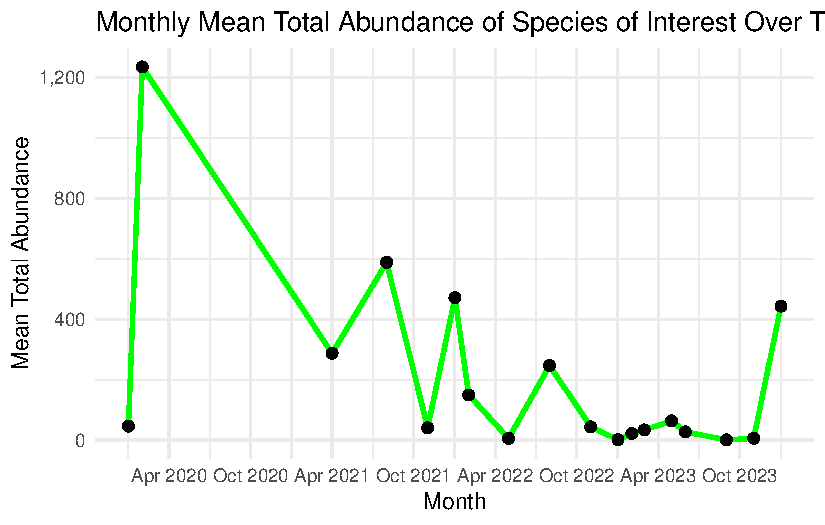
\includegraphics[keepaspectratio]{timeline-check-in_files/figure-pdf/exp. fig 3 - time-series plot of total abundance-1.pdf}}

Clarification: To reduce visual clutter from sampling dates that
occurred close together, total abundance was first calculated for each
sampling date and then averaged within each month. This monthly summary
makes broader temporal patterns easier to interpret than plotting every
individual sampling date.

Description of visual components

This figure shows total abundance of the focus invertebrate taxa over
time. Each black point represents one sampling date, where abundance was
summed across all sites and across all taxa of interest. The green line
connects sampling dates in chronological order to show changes in total
abundance over time. The x-axis shows sampling date, and the y-axis
shows total abundance.

Main message / takeaway

Total invertebrate abundance varies substantially over time, with one
very large peak in 2020 and several smaller peaks in later years. There
is no consistent increasing or decreasing trend across the full time
period. Abundance appears highly variable among sampling dates.

Connection to the main question

This figure provides context for the dissolved oxygen and invertebrate
abundance relationship by showing that abundance changes strongly across
sampling dates. This is important because variation over time may
influence observed abundance patterns in addition to dissolved oxygen
levels.

\subsection{Exploratory Figure 4: Time-series area
plot}\label{exploratory-figure-4-time-series-area-plot}

\begin{Shaded}
\begin{Highlighting}[]
\CommentTok{\# create object taxon\_abundance\_time from DO\_taxa}
\NormalTok{taxon\_abundance\_time }\OtherTok{\textless{}{-}}\NormalTok{ DO\_taxa }\SpecialCharTok{|\textgreater{}}
  \CommentTok{\# keeps only the focus taxa}
  \FunctionTok{filter}\NormalTok{(taxon }\SpecialCharTok{\%in\%}\NormalTok{ focus\_taxa) }\SpecialCharTok{|\textgreater{}}
  \CommentTok{\# makes sure date is treated as a Date object}
  \FunctionTok{mutate}\NormalTok{(}\AttributeTok{date =} \FunctionTok{as.Date}\NormalTok{(date)) }\SpecialCharTok{|\textgreater{}}
  \CommentTok{\# creates a month column}
  \FunctionTok{mutate}\NormalTok{(}\AttributeTok{month =}\NormalTok{ lubridate}\SpecialCharTok{::}\FunctionTok{floor\_date}\NormalTok{(date, }\AttributeTok{unit =} \StringTok{"month"}\NormalTok{)) }\SpecialCharTok{|\textgreater{}}
  \CommentTok{\# groups by date, month, and taxon }
  \FunctionTok{group\_by}\NormalTok{(date, month, taxon) }\SpecialCharTok{|\textgreater{}}
  \CommentTok{\# sums abundance across sites for each taxon on each sampling date}
  \FunctionTok{summarise}\NormalTok{(}
    \CommentTok{\# calculates total abundance per taxon for each sampling date}
    \AttributeTok{daily\_taxon\_abundance =} \FunctionTok{sum}\NormalTok{(ave\_lit, }\AttributeTok{na.rm =} \ConstantTok{TRUE}\NormalTok{),}
    \CommentTok{\# ungroup}
    \AttributeTok{.groups =} \StringTok{"drop"}\NormalTok{) }\SpecialCharTok{|\textgreater{}}
  \CommentTok{\# groups by month and taxon}
  \FunctionTok{group\_by}\NormalTok{(month, taxon) }\SpecialCharTok{|\textgreater{}}
  \CommentTok{\# calculates monthly mean abundance for each taxon}
  \FunctionTok{summarise}\NormalTok{(}
    \CommentTok{\# averages taxon abundance across sampling dates within each month}
    \AttributeTok{monthly\_taxon\_abundance =} \FunctionTok{mean}\NormalTok{(daily\_taxon\_abundance, }\AttributeTok{na.rm =} \ConstantTok{TRUE}\NormalTok{),}
    \CommentTok{\# ungroup}
    \AttributeTok{.groups =} \StringTok{"drop"}\NormalTok{) }\SpecialCharTok{|\textgreater{}}
  \CommentTok{\# groups by month }
  \FunctionTok{group\_by}\NormalTok{(month) }\SpecialCharTok{|\textgreater{}}
  \CommentTok{\# calculates each taxon\textquotesingle{}s proportion of total monthly abundance}
  \FunctionTok{mutate}\NormalTok{(}\CommentTok{\# divides each taxon\textquotesingle{}s monthly abundance by the total abundance per month}
    \AttributeTok{proportion =}\NormalTok{ monthly\_taxon\_abundance }\SpecialCharTok{/} \FunctionTok{sum}\NormalTok{(monthly\_taxon\_abundance)) }\SpecialCharTok{|\textgreater{}}
  \CommentTok{\# ungroup}
  \FunctionTok{ungroup}\NormalTok{()}

\CommentTok{\# create time series area plot using taxon\_abundance\_time df}
\FunctionTok{ggplot}\NormalTok{(taxon\_abundance\_time,}
       \FunctionTok{aes}\NormalTok{(}\AttributeTok{x =}\NormalTok{ month, }\CommentTok{\# x{-}axis is month}
           \AttributeTok{y =}\NormalTok{ proportion, }\CommentTok{\# y{-}axis is proportion}
           \AttributeTok{fill =}\NormalTok{ taxon)) }\SpecialCharTok{+} \CommentTok{\# fill color by taxon}
  \CommentTok{\# creates stacked area plot where total height is 100\% of abundance per month}
  \FunctionTok{geom\_area}\NormalTok{(}\AttributeTok{alpha =} \FloatTok{0.8}\NormalTok{) }\SpecialCharTok{+} \CommentTok{\# sets opacity}
  \CommentTok{\# formats y{-}axis as percentages and keeps limits from 0\% to 100\%}
  \FunctionTok{scale\_y\_continuous}\NormalTok{(}\AttributeTok{labels =}\NormalTok{ scales}\SpecialCharTok{::}\FunctionTok{percent\_format}\NormalTok{(), }\AttributeTok{limits =} \FunctionTok{c}\NormalTok{(}\DecValTok{0}\NormalTok{, }\DecValTok{1}\NormalTok{)) }\SpecialCharTok{+}
  \CommentTok{\# formats x{-}axis dates so monthly time patterns are easier to read}
  \FunctionTok{scale\_x\_date}\NormalTok{(}\AttributeTok{date\_breaks =} \StringTok{"6 months"}\NormalTok{, }\AttributeTok{date\_labels =} \StringTok{"\%b \%Y"}\NormalTok{) }\SpecialCharTok{+}
  \CommentTok{\# adds clear labels}
  \FunctionTok{labs}\NormalTok{(}
    \CommentTok{\# creates descriptive title}
    \AttributeTok{title =} \StringTok{"Relative Abundance of Species of Interest Over Time"}\NormalTok{,}
    \AttributeTok{x =} \StringTok{"Month"}\NormalTok{, }\CommentTok{\# labels x{-}axis}
    \AttributeTok{y =} \StringTok{"Proportion of Monthly Abundance"}\NormalTok{, }\CommentTok{\# labels y{-}axis}
    \AttributeTok{fill =} \StringTok{"Taxon"}\NormalTok{) }\SpecialCharTok{+}\CommentTok{\# labels fill legend}
  \CommentTok{\# uses non{-}default theme}
  \FunctionTok{theme\_minimal}\NormalTok{() }\SpecialCharTok{+}
  \CommentTok{\# rotates x{-}axis text to make month labels easier to read}
  \FunctionTok{theme}\NormalTok{(}\AttributeTok{axis.text.x =} \FunctionTok{element\_text}\NormalTok{(}\AttributeTok{angle =} \DecValTok{45}\NormalTok{, }\AttributeTok{hjust =} \DecValTok{1}\NormalTok{))}
\end{Highlighting}
\end{Shaded}

\pandocbounded{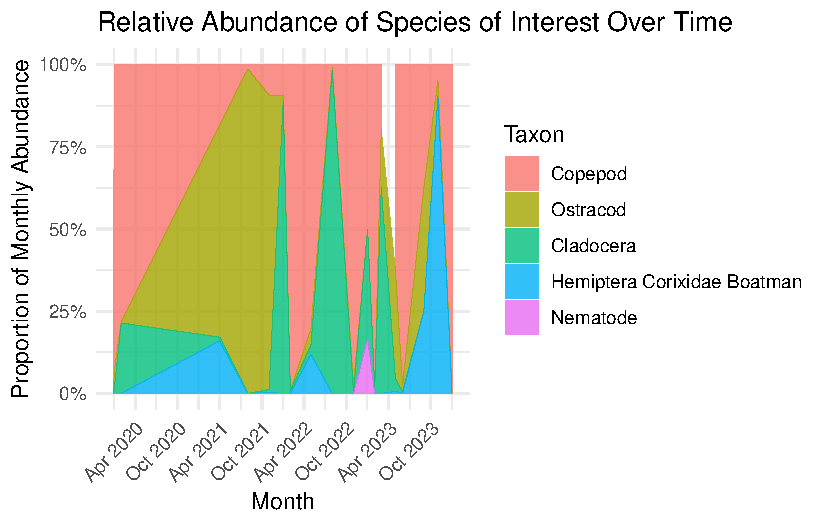
\includegraphics[keepaspectratio]{timeline-check-in_files/figure-pdf/exp. figure 4 - Time-series area plot-1.pdf}}

To make the time series easier to interpret, abundance was summarized by
month rather than plotted for every individual sampling date. The
stacked area plot shows the proportional contribution of each taxon to
total monthly abundance, so the y-axis ranges from 0\% to 100\% and
highlights changes in community composition over time.

Description of visual components

This figure shows changes in abundance over time for our five focus
invertebrate taxa: Ostracod, Copepod, Cladocera, Hemiptera Corixidae
Boatman, and Nematode. Each different colored area represents the summed
average abundance per liter for one taxon on each sampling date, summed
across sites but kept separate by taxon. The stacked height of the
colored areas represents the total abundance of all focus taxa combined
at that sampling date. The x-axis shows sampling date, and the y-axis
shows average abundance per liter.

Main message / takeaway

Abundance varies strongly over time, and different taxa contribute to
peaks at different points. Copepods appear to drive the largest peak in
2020 and another increase near 2024, while Ostracods and Cladocera
contribute noticeably to some intermediate peaks.

Connection to the main question

This figure adds time and taxon-specific context to the relationship
between dissolved oxygen and invertebrate abundance. It shows that
abundance patterns are not constant over time and that changes in total
abundance may be driven by shifts in particular taxa, which is important
when interpreting how the community responds to DO conditions.

\subsection{Exploratory Figure 5: Distribution of Median Dissolved
Oxygen Aross
Sites}\label{exploratory-figure-5-distribution-of-median-dissolved-oxygen-aross-sites}

\begin{Shaded}
\begin{Highlighting}[]
\CommentTok{\# create new object to store medians of median do levels}
\NormalTok{median\_fig2 }\OtherTok{\textless{}{-}}\NormalTok{ aq\_ins\_clean\_fig2 }\SpecialCharTok{|\textgreater{}} 
  \FunctionTok{group\_by}\NormalTok{(site\_full) }\SpecialCharTok{|\textgreater{}} 
  \FunctionTok{summarize}\NormalTok{(}\AttributeTok{median\_do =} \FunctionTok{median}\NormalTok{(med\_do, }\AttributeTok{na.rm =} \ConstantTok{TRUE}\NormalTok{))}

\CommentTok{\# assign quartiles for each site}
\NormalTok{aq\_ins\_clean\_fig2}\SpecialCharTok{$}\NormalTok{quartile }\OtherTok{\textless{}{-}} \FunctionTok{cut}\NormalTok{(}
\NormalTok{  aq\_ins\_clean\_fig2}\SpecialCharTok{$}\NormalTok{med\_do, }
  \AttributeTok{breaks =} \FunctionTok{quantile}\NormalTok{(aq\_ins\_clean\_fig2}\SpecialCharTok{$}\NormalTok{med\_do, }\AttributeTok{na.rm =} \ConstantTok{TRUE}\NormalTok{, }\AttributeTok{probs =} \FunctionTok{seq}\NormalTok{(}\DecValTok{0}\NormalTok{, }\DecValTok{1}\NormalTok{, }\FloatTok{0.25}\NormalTok{)), }
  \AttributeTok{labels =} \FunctionTok{c}\NormalTok{(}\StringTok{"Q1"}\NormalTok{, }\StringTok{"Q2"}\NormalTok{, }\StringTok{"Q3"}\NormalTok{, }\StringTok{"Q4"}\NormalTok{), }
  \AttributeTok{include.lowest =} \ConstantTok{TRUE}\NormalTok{,}
  \AttributeTok{right =} \ConstantTok{FALSE}\NormalTok{)}

\CommentTok{\# boundaries of quartiles}
\NormalTok{q }\OtherTok{\textless{}{-}} \FunctionTok{quantile}\NormalTok{(aq\_ins\_clean\_fig2}\SpecialCharTok{$}\NormalTok{med\_do, }\AttributeTok{na.rm =} \ConstantTok{TRUE}\NormalTok{, }\AttributeTok{probs =} \FunctionTok{seq}\NormalTok{(}\DecValTok{0}\NormalTok{, }\DecValTok{1}\NormalTok{, }\FloatTok{0.25}\NormalTok{))}

\FunctionTok{view}\NormalTok{(q)}

\NormalTok{dens }\OtherTok{\textless{}{-}} \FunctionTok{density}\NormalTok{(aq\_ins\_clean\_fig2}\SpecialCharTok{$}\NormalTok{med\_do, }\AttributeTok{na.rm =} \ConstantTok{TRUE}\NormalTok{)}

\CommentTok{\# one row per site}
\NormalTok{label\_df }\OtherTok{\textless{}{-}}\NormalTok{ aq\_ins\_clean\_fig2 }\SpecialCharTok{|\textgreater{}} 
  \FunctionTok{group\_by}\NormalTok{(site\_full) }\SpecialCharTok{|\textgreater{}} 
  \FunctionTok{summarize}\NormalTok{(}\AttributeTok{median\_do =} \FunctionTok{median}\NormalTok{(med\_do, }\AttributeTok{na.rm =} \ConstantTok{TRUE}\NormalTok{))}

\CommentTok{\# approximate density height for each site}
\NormalTok{label\_df}\SpecialCharTok{$}\NormalTok{y }\OtherTok{\textless{}{-}} \FunctionTok{approx}\NormalTok{(}
\NormalTok{  dens}\SpecialCharTok{$}\NormalTok{x,}
\NormalTok{  dens}\SpecialCharTok{$}\NormalTok{y,}
  \AttributeTok{xout =}\NormalTok{ label\_df}\SpecialCharTok{$}\NormalTok{median\_do}
\NormalTok{)}\SpecialCharTok{$}\NormalTok{y}

\CommentTok{\# distribution plot of DO levels across sites}
\FunctionTok{ggplot}\NormalTok{(aq\_ins\_clean\_fig2, }\FunctionTok{aes}\NormalTok{(}\AttributeTok{x =}\NormalTok{ med\_do)) }\SpecialCharTok{+}
  \CommentTok{\# density curve}
  \FunctionTok{geom\_density}\NormalTok{(}\AttributeTok{fill =} \StringTok{"lightblue"}\NormalTok{,}
               \AttributeTok{alpha =} \FloatTok{0.4}\NormalTok{,}
               \AttributeTok{color =} \StringTok{"blue"}\NormalTok{,}
               \AttributeTok{linewidth =} \FloatTok{1.2}\NormalTok{) }\SpecialCharTok{+}
  \CommentTok{\# vertical quartile lines}
  \FunctionTok{geom\_vline}\NormalTok{(}\AttributeTok{xintercept =}\NormalTok{ q,}
             \AttributeTok{linetype =} \StringTok{"dashed"}\NormalTok{,}
             \AttributeTok{color =} \StringTok{"gray40"}\NormalTok{) }\SpecialCharTok{+}
  \CommentTok{\# segments pointing to sites}
   \FunctionTok{geom\_segment}\NormalTok{(}
    \AttributeTok{data =}\NormalTok{ label\_df,}
    \FunctionTok{aes}\NormalTok{(}
      \AttributeTok{x =}\NormalTok{ median\_do,}
      \AttributeTok{xend =}\NormalTok{ median\_do,}
      \AttributeTok{y =} \DecValTok{0}\NormalTok{,}
      \AttributeTok{yend =} \FloatTok{0.015}
\NormalTok{    ),}
    \AttributeTok{color =} \StringTok{"gray40"}
\NormalTok{  ) }\SpecialCharTok{+}
  \CommentTok{\# site labels}
  \FunctionTok{geom\_text}\NormalTok{(}
    \AttributeTok{data =}\NormalTok{ label\_df,}
    \FunctionTok{aes}\NormalTok{(}
      \AttributeTok{x =}\NormalTok{ median\_do,}
      \AttributeTok{y =} \FloatTok{0.018}\NormalTok{,}
      \AttributeTok{label =} \FunctionTok{str\_wrap}\NormalTok{(site\_full, }\AttributeTok{width =} \DecValTok{10}\NormalTok{)}
\NormalTok{    ),}
    \AttributeTok{size =} \DecValTok{3}
\NormalTok{  ) }\SpecialCharTok{+}
  \CommentTok{\# quartile dashed line labels}
  \FunctionTok{geom\_text}\NormalTok{(}\AttributeTok{data =} \FunctionTok{data.frame}\NormalTok{(}\AttributeTok{x =}\NormalTok{ q, }\AttributeTok{label =} \FunctionTok{names}\NormalTok{(q)), }
            \FunctionTok{aes}\NormalTok{(}\AttributeTok{x =}\NormalTok{ x, }\AttributeTok{y =} \FloatTok{0.14}\NormalTok{, }\AttributeTok{label =} \FunctionTok{paste0}\NormalTok{(label, }\StringTok{"}\SpecialCharTok{\textbackslash{}n}\StringTok{"}\NormalTok{, }\FunctionTok{round}\NormalTok{(x, }\DecValTok{2}\NormalTok{))),}
            \AttributeTok{color =} \StringTok{"gray40"}\NormalTok{,}
            \AttributeTok{size =} \FloatTok{3.5}\NormalTok{,}
            \AttributeTok{hjust =} \SpecialCharTok{{-}}\FloatTok{0.1}\NormalTok{) }\SpecialCharTok{+} \CommentTok{\# shift text slightly to the right of the line}
  \CommentTok{\# remove space between bottom of plot and y{-}axis, set y{-}axis limits}
  \FunctionTok{scale\_y\_continuous}\NormalTok{(}\AttributeTok{expand =} \FunctionTok{c}\NormalTok{(}\DecValTok{0}\NormalTok{,}\DecValTok{0}\NormalTok{),}
                     \AttributeTok{limits =} \FunctionTok{c}\NormalTok{(}\DecValTok{0}\NormalTok{, }\FloatTok{0.15}\NormalTok{)) }\SpecialCharTok{+}
  \CommentTok{\# axes labels and title}
  \FunctionTok{labs}\NormalTok{(}\AttributeTok{x =} \StringTok{"Median Dissolved Oxygen (mg/L)"}\NormalTok{,}
       \AttributeTok{y =} \StringTok{"Density"}\NormalTok{,}
       \AttributeTok{title =} \StringTok{"Distribution of Median Dissolved Oxygen Aross Sites"}\NormalTok{) }\SpecialCharTok{+}
  \CommentTok{\# theme}
  \FunctionTok{theme\_bw}\NormalTok{() }\SpecialCharTok{+}
  \CommentTok{\# remove legend}
  \FunctionTok{theme}\NormalTok{(}\AttributeTok{legend.position =} \StringTok{"none"}\NormalTok{)}
\end{Highlighting}
\end{Shaded}

\pandocbounded{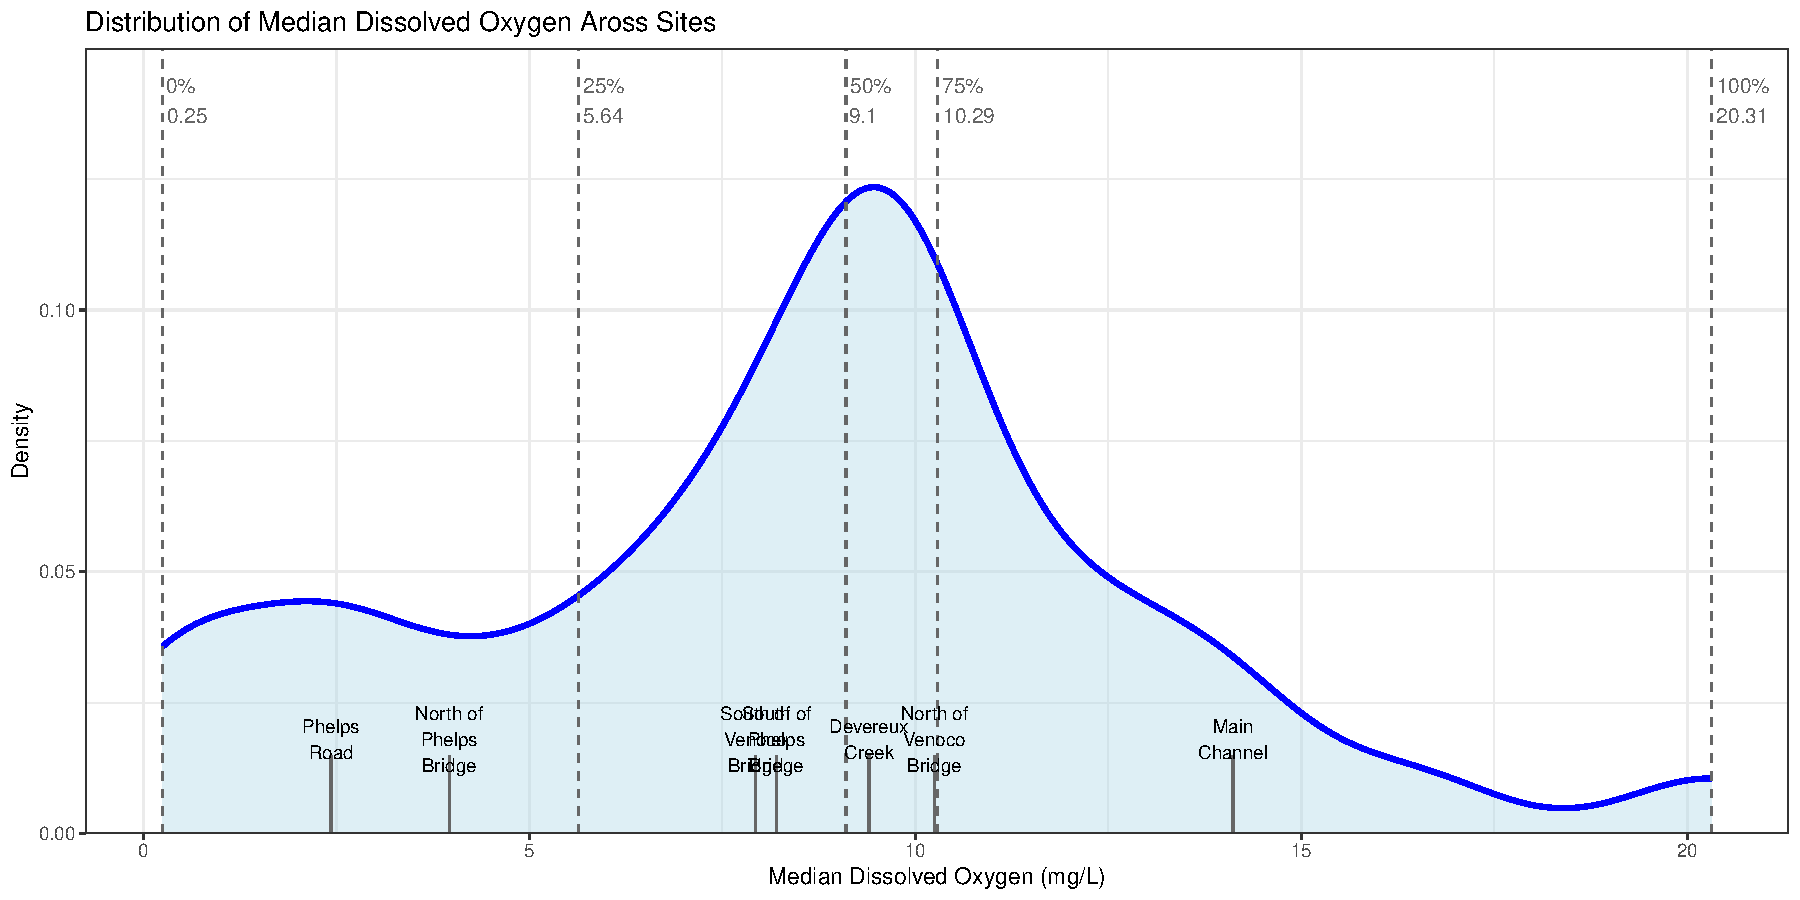
\includegraphics[keepaspectratio]{timeline-check-in_files/figure-pdf/do-vs-sites-bins-1.pdf}}

These bins were created by according to the median dissolved oxygen
levels at each site. Low DO is the 25th percentile, moderate DO is the
75th percentile, and high DO is the 100th percentile. The labels show
the median of the median DO measurments at each site.

\begin{itemize}
\tightlist
\item
  Low DO: Phelps Road and North of Phelps Bridge
\item
  Moderate DO: South of Venoco Bridge, South of Phelps Bridge, Devereux
  Creek, North of Venoco Bridge
\item
  High DO: Main Channel
\end{itemize}

Description of visual components

This figure shows the distribution of median dissolved oxygen values
across the invertebrate sampling observations. The blue density curve
shows where DO values are most concentrated, with higher areas of the
curve indicating more observations at those DO levels. The dashed
vertical lines mark the minimum, 25th percentile, median, 75th
percentile, and maximum DO values, which are used to understand the
spread of DO conditions. The site labels and short vertical gray lines
near the bottom show the median DO value for each site. This allows
site-level DO conditions to be easily compared.

Main message / takeaway

Median DO values are mostly concentrated around roughly 8--11 mg/L, but
there is a wide overall range from very low DO values to values above 20
mg/L. Sites differ in their typical DO levels, with Phelps Road and
North of Phelps Bridge having relatively low median DO, while Main
Channel has a higher median DO.

Connection to the main question

This figure helps contextualize the main question by showing the range
of dissolved oxygen conditions that invertebrates experienced across
sites. It also supports the use of low, medium, and high DO categories
by showing where the quartile cutoffs occur within the DO distribution.

\subsection{Exploratory Figure 6: Invertebrate Abundance in DO
Bins}\label{exploratory-figure-6-invertebrate-abundance-in-do-bins}

\begin{Shaded}
\begin{Highlighting}[]
\CommentTok{\# base layer: ggplot}
\NormalTok{ins\_bins\_plot }\OtherTok{\textless{}{-}} \FunctionTok{ggplot}\NormalTok{(}\AttributeTok{data =}\NormalTok{ aq\_ins\_clean\_bins, }
                        \AttributeTok{mapping =} \FunctionTok{aes}\NormalTok{(}\AttributeTok{x =}\NormalTok{ bins, }\CommentTok{\# x{-}axis: DO bins}
                                      \AttributeTok{y =}\NormalTok{ log\_ave\_lit, }\CommentTok{\# y{-}axis: log\_ave\_lit}
                                      \AttributeTok{color =}\NormalTok{ taxon)) }\SpecialCharTok{+} \CommentTok{\# color by taxon}
  \CommentTok{\# first layer: points show individual abundance measurements }
  \FunctionTok{geom\_jitter}\NormalTok{(}\AttributeTok{width =} \FloatTok{0.15}\NormalTok{,}
              \AttributeTok{height =} \DecValTok{0}\NormalTok{,}
              \AttributeTok{shape =} \DecValTok{16}\NormalTok{,}
              \AttributeTok{size =} \DecValTok{2}\NormalTok{,}
            \AttributeTok{alpha =} \FloatTok{0.7}\NormalTok{) }\SpecialCharTok{+}
  \CommentTok{\# calculate median for each bin for each taxon}
  \FunctionTok{stat\_summary}\NormalTok{(}\AttributeTok{fun =}\NormalTok{ median,}
               \AttributeTok{geom =} \StringTok{"point"}\NormalTok{,}
               \AttributeTok{color =} \StringTok{"red"}\NormalTok{,}
               \AttributeTok{size =} \DecValTok{3}\NormalTok{) }\SpecialCharTok{+}
  \CommentTok{\# separate panels for each taxon }
  \FunctionTok{facet\_wrap}\NormalTok{(}\SpecialCharTok{\textasciitilde{}}\NormalTok{ taxon) }\SpecialCharTok{+}
  \CommentTok{\# use non{-}default colors for points}
  \FunctionTok{scale\_color\_viridis\_d}\NormalTok{() }\SpecialCharTok{+}
  \FunctionTok{labs}\NormalTok{(}\AttributeTok{x =} \StringTok{"DO levels"}\NormalTok{, }\CommentTok{\# relabel x{-}axis}
       \AttributeTok{y =} \StringTok{"log + 1 transformed average abundance/L"}\NormalTok{, }\CommentTok{\# relabel y{-}axis}
       \CommentTok{\# creates descriptive title}
       \AttributeTok{title =} \StringTok{"Invertebrate abundance vs DO levels"}\NormalTok{) }\SpecialCharTok{+}
  \CommentTok{\# uses non{-}default theme}
  \FunctionTok{theme\_bw}\NormalTok{() }\SpecialCharTok{+}
  \CommentTok{\# remove redundant legend}
  \FunctionTok{theme}\NormalTok{(}\AttributeTok{legend.position =} \StringTok{"none"}\NormalTok{)}

\CommentTok{\# shows plot}
\NormalTok{ins\_bins\_plot}
\end{Highlighting}
\end{Shaded}

\pandocbounded{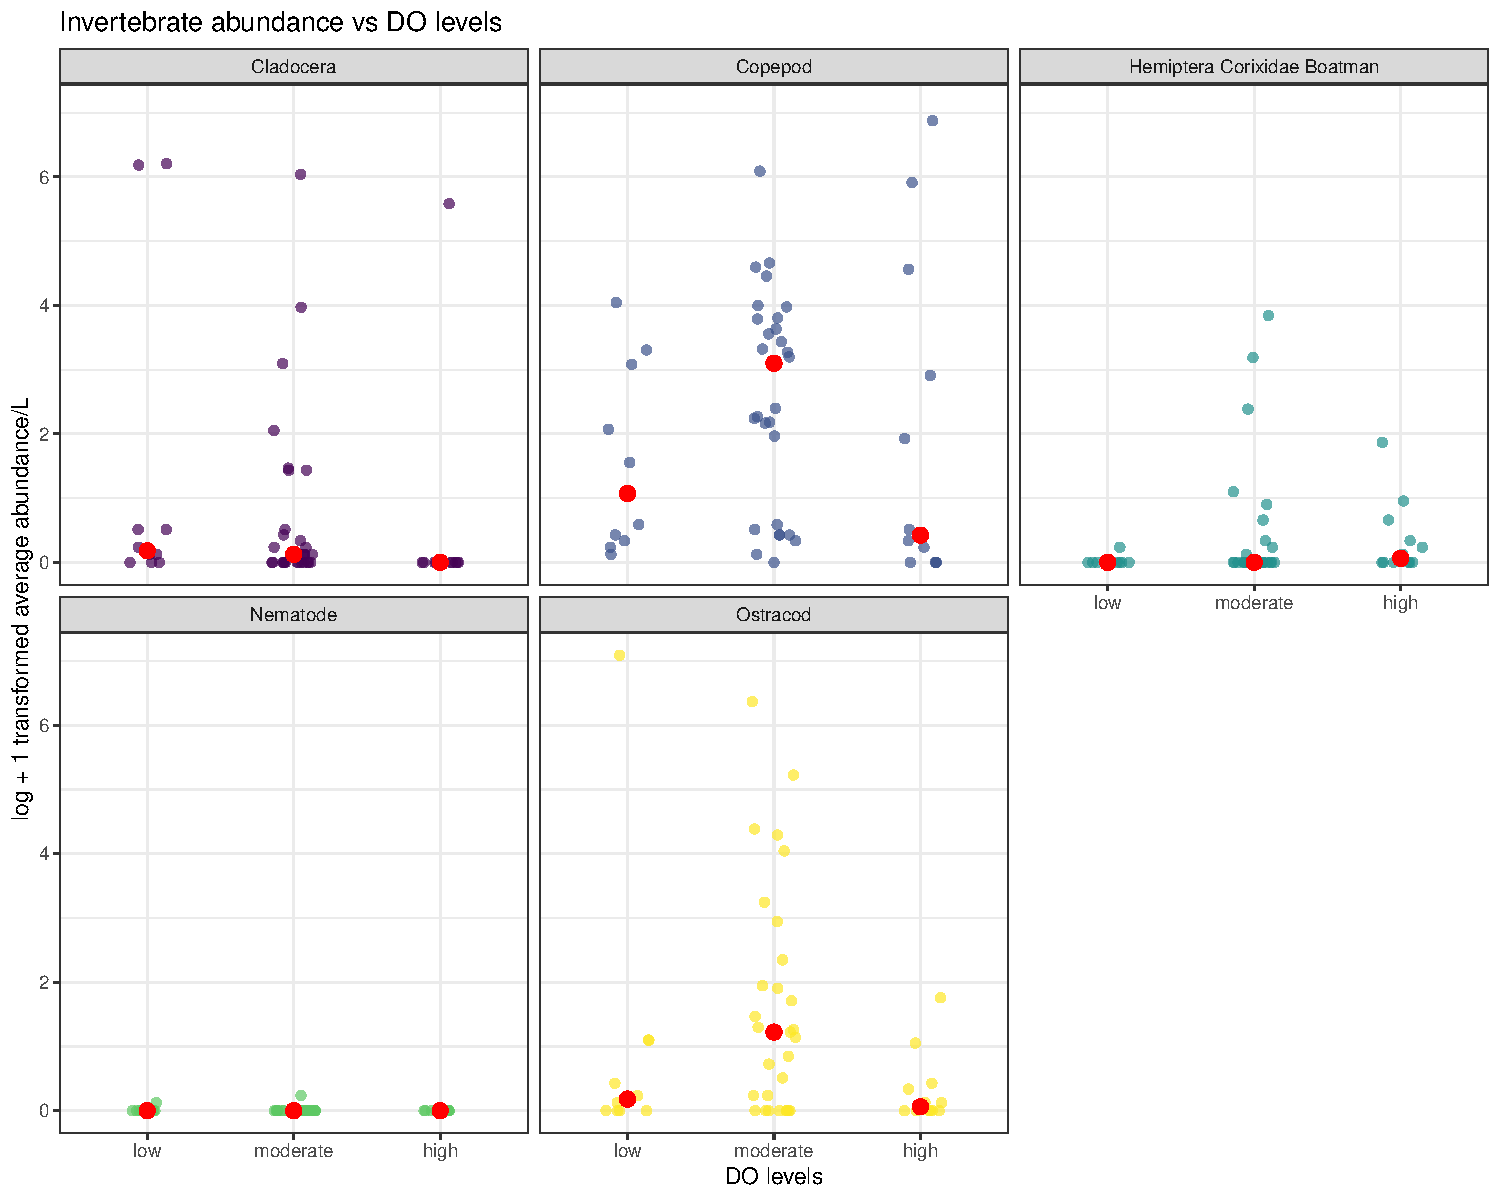
\includegraphics[keepaspectratio]{timeline-check-in_files/figure-pdf/invert-abundance-at-bins-1.pdf}}

Description of visual components

This figure shows taxon-specific invertebrate abundance across the three
dissolved oxygen categories: low, moderate, and high. Each panel
represents one focus taxon. Each small colored point represents one
sampling observation for that taxon, with the x-axis showing the DO
category and the y-axis showing log + 1 transformed average abundance
per liter. The large red points represent the median abundance for each
taxon within each DO category.

Main message / takeaway

The figure suggests that the relationship between abundance and DO level
differs among taxa rather than following one single community-wide
pattern. Copepods and Ostracods tend to show higher and more variable
abundances in the moderate DO category, while Nematodes remain near zero
across all DO levels and Hemiptera Corixidae Boatman abundace stays
generally low with only a few higher values at moderate DO.

Connection to the main question

This figure helps address the main question by showing whether
individual invertebrate taxa respond differently across dissolved oxygen
conditions. It adds important context by demonstrating that DO effects
may be taxon-specific, meaning patterns in total abundance could be
driven by stronger responses in some groups than in others.

\section{Plan for elective}\label{plan-for-elective}

Draft 1:

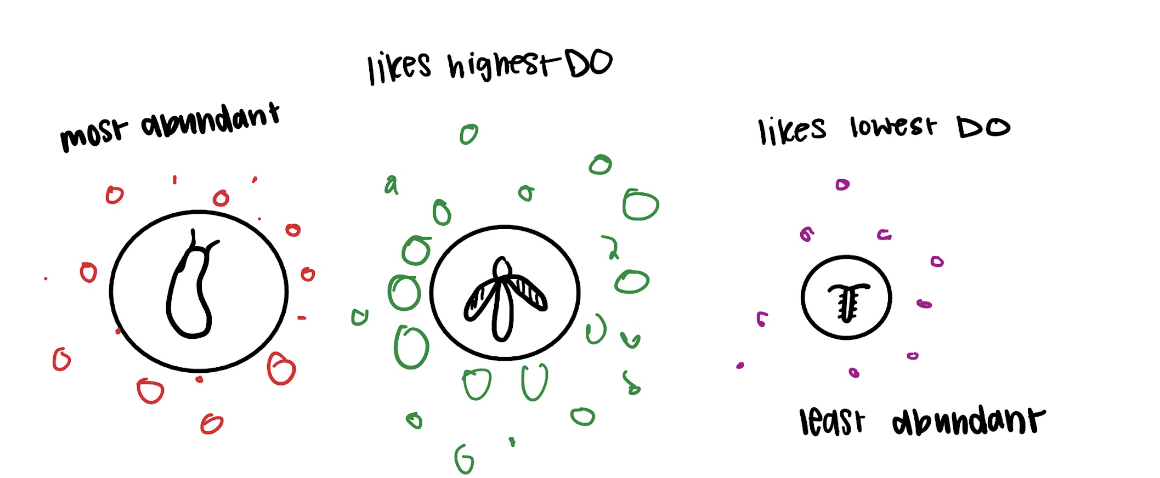
\includegraphics[width=0.7\linewidth,height=\textheight,keepaspectratio]{draft_elective.png}

Draft 2:

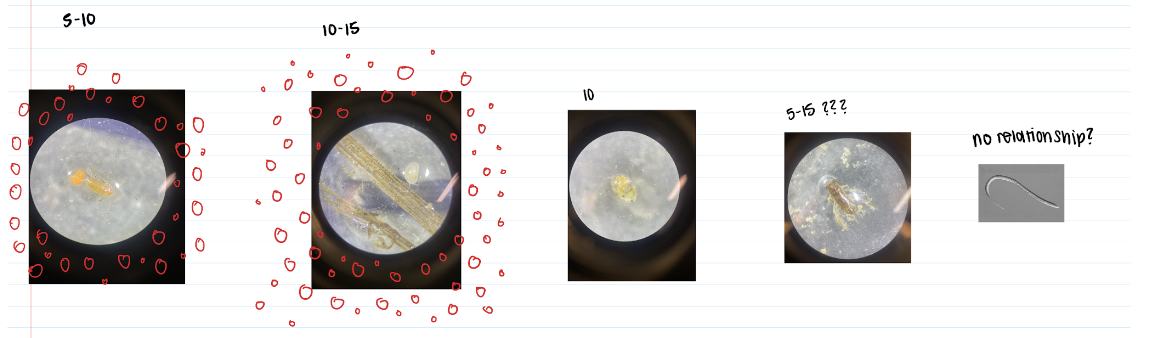
\includegraphics[width=0.7\linewidth,height=\textheight,keepaspectratio]{new_draft_elective.png}

Focus Taxa Images:

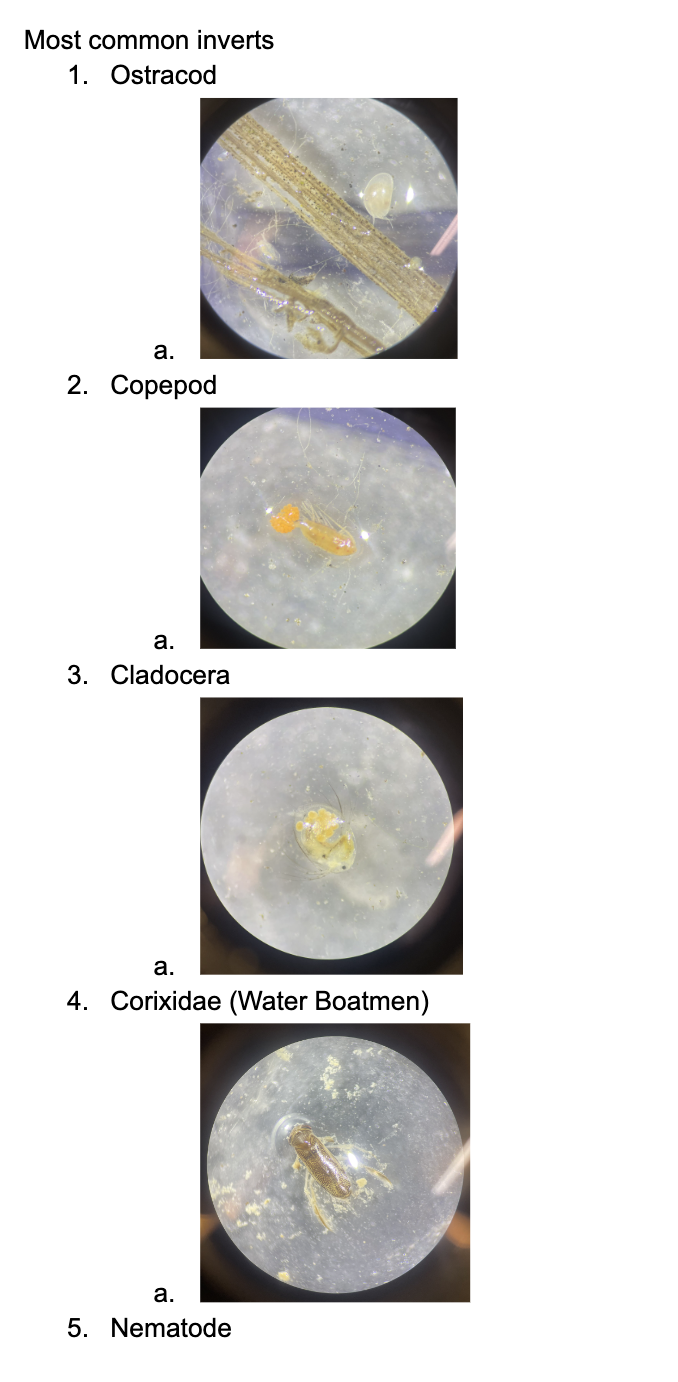
\includegraphics[width=0.3\linewidth,height=\textheight,keepaspectratio]{elective_images.png}

\textbf{Elective idea general concept: } Our elective aims to show
several factors we examined for the relationship between NCOS aquatic
inverts and dissolved oxygen. Using the size of the microscopic images
of each of the 5 main invert species, we are able to display abundance.
The larger the picture, the more abundant that species is. We then plan
to paint watercolor bubbles around each invert to show each species
preferred DO levels.

\textbf{Progress we have made}: Each of the microscopic images were
collected through samples at the NCOS lab (with the exception of
nematodes) for this elective. Another large area of progress that has
been made is actually figuring out what the relationship between each
invert and DO is. We found that there is little to no correlation
between these two factors and that each invert prefers similar low
levels of DO.

\textbf{Possible changes that should be made based on our findings}:
Rather than bubbles representing each species proffered amount of DO,
the bubbles could represent the strength of the relationship between the
species abundance and the DO levels. For species with a negative
correlation, we could draw the bubbles a different color.




\end{document}
